\documentclass[12pt,a4paper]{article}

\usepackage[utf8]{inputenc}
\usepackage[T1]{fontenc}
\usepackage{amsmath,amssymb,amsfonts,amsthm}
\usepackage{mathtools}
\usepackage{booktabs}
\usepackage{graphicx}
\usepackage[shortlabels]{enumitem}
\usepackage[margin=2.5cm]{geometry}
\usepackage[numbers,sort&compress]{natbib}
\usepackage{doi}
\usepackage{xcolor}
\usepackage{float}
\usepackage{hyperref}
\usepackage{array}
\usepackage{multirow}

\hypersetup{
  colorlinks=true,
  linkcolor=blue!60!black,
  citecolor=blue!60!black,
  urlcolor=blue!60!black,
  pdfauthor={David Alfyorov, Igor Shnyukov},
  pdftitle={Weyl curvature from the Hasse diagram: a parameter-free bridge formula for causal sets},
  pdfsubject={gr-qc}
}

% --- Theorem environments ---
\theoremstyle{plain}
\newtheorem{theorem}{Theorem}[section]
\newtheorem{proposition}[theorem]{Proposition}
\newtheorem{lemma}[theorem]{Lemma}
\newtheorem{corollary}[theorem]{Corollary}
\theoremstyle{definition}
\newtheorem{definition}[theorem]{Definition}
\newtheorem{condition}[theorem]{Condition}
\theoremstyle{remark}
\newtheorem{remark}[theorem]{Remark}
\newtheorem{example}[theorem]{Example}

% --- Custom commands ---
\newcommand{\dd}{\mathrm{d}}
\newcommand{\Tr}{\operatorname{Tr}}
\newcommand{\tr}{\operatorname{tr}}
\newcommand{\Cov}{\operatorname{Cov}}
\newcommand{\Var}{\operatorname{Var}}
\newcommand{\erfi}{\operatorname{erfi}}
\newcommand{\order}{\mathcal{O}}
\newcommand{\Esq}{E_{ij}E^{ij}}
\newcommand{\CJ}{\mathrm{CJ}}

\graphicspath{{figures/}}

\title{Weyl curvature from the Hasse diagram:\\
a parameter-free bridge formula for causal sets}
\author{David Alfyorov, Igor Shnyukov\\[4pt]
\small\textit{davidich.alfyorov@gmail.com}}
\date{March 2026}

\begin{document}
\maketitle

% ============================================================
\begin{abstract}
% ============================================================

We construct a statistical estimator on Poisson-sprinkled causal
sets in four spacetime dimensions and derive, both analytically
and numerically, a parameter-free relationship between this
estimator and the electric part of the Weyl tensor.  The
estimator, denoted~$\CJ$, is a stratified covariance of
path-count observables computed from the Hasse diagram.  On a
vacuum causal diamond of proper time~$T$ with $N$~sprinkled
elements, we find
\begin{equation}\label{eq:bridge-abstract}
  \langle \CJ \rangle
  = 4 \cdot \frac{8}{3} \cdot \frac{1}{9!}
    \cdot \frac{8\pi}{15} \cdot \frac{\pi}{24}
    \cdot N^{8/9}\, \Esq\, T^4,
\end{equation}
where each factor has a distinct geometric origin: $4 = 2^2$
from the two-leg structure of the link score, $8/3 = c_4^2$
from the squared Benincasa--Dowker normalisation, $1/9!$ from
the nine-simplex beta overlap, $8\pi/15$ from the angular
average of the squared tidal deformation, and $\pi/24$ from
the four-dimensional diamond volume.  The combined numerical
prefactor is $C_0 = 32\pi^2/(3 \cdot 9! \cdot 45)
\approx 6.44 \times 10^{-6}$.  The rational coefficient contains no continuous free parameters;
the factor~$4 = 2^2$ is derived from the two-leg structure of the
link score in the bulk regime, and the exponent~$8/9$ is
empirically established but not derived from first principles.

The formula is verified against Monte Carlo data on exact pp-wave
causal diamonds for $N = 500$--$15{,}000$: the ratio of measured
to predicted CJ is $1.016 \pm 0.015$, with residual scatter
below~$4\%$.  Seven independent diagnostic tests are reported,
including a de~Sitter null test ($\CJ = 0$ exactly), Kottler
cross-term, polarisation dependence, and Sorkin--Johnston entropy
independence.  The derivation rests on two explicitly stated
conditions concerning the continuum limit of the stratified
estimator.  The $N^{8/9}$ exponent is empirically established
but not derived from first principles.  All rational coefficient
identities, including the general-$d$ beta overlap
$(d!)^2\binom{2d}{d}(2d+1) = (2d+1)!$, are formally verified
in Lean~4 using the Mathlib library (105~sorry-free theorems).
Five failed approaches and thirty closed spectral routes are
documented.

\end{abstract}

\tableofcontents
\newpage

% ============================================================
\section{Introduction}
\label{sec:intro}
% ============================================================

A central question in causal set theory is how continuum geometric
quantities emerge from the discrete causal order.  The causal set
programme, initiated by Bombelli, Lee, Meyer, and
Sorkin~\cite{Bombelli:1987aa}, with precursors in the work of
Myrheim~\cite{Myrheim:1978} and 't~Hooft~\cite{tHooft:1979},
posits that spacetime at the Planck scale is a locally finite
partially ordered set whose order relation encodes the causal
structure.  The continuum spacetime is recovered in a suitable
large-$N$ limit, and physical observables are functions of the
partial order that approximate continuum geometric
invariants~\cite{Surya:2019ndm}.

Significant progress has been made at the level of the scalar
curvature.  The Benincasa--Dowker (BD) action~\cite{BenincasaDowker:2010}
provides a causal-set estimator whose continuum limit yields the
integrated Ricci scalar $\int R\sqrt{-g}\,\dd^4x$, with the
four-dimensional normalisation coefficient $c_4 = 4/\sqrt{6}$
established in~\cite{BenincasaDowker:2010,Belenchia:2015}.
Roy, Sinha, and Surya~\cite{RoySinhaSurya:2013} showed that
chain-counting observables extract the Ricci scalar to leading
order in the small-diamond expansion.  At the next order,
Benincasa, Dowker, and Glaser~\cite{BenincasaDowkerGlaser:2011}
studied the random discrete action in two dimensions.  More
recently, de~Brito, Eichhorn, and Pfeiffer~\cite{deBrito:2023}
demonstrated that the squared BD operator converges in the
continuum to the combination $R^2 - 2\Box R$, using stacked
order intervals that go beyond ordinary Alexandrov diamonds.

At the Weyl-squared level, however, no discrete observable has
previously been shown to converge to any Weyl invariant.  On the
continuum side, Wang~\cite{Wang:2019} established that the volume
deficit of the Alexandrov diamond is proportional
to~$\Esq$ specifically in four dimensions, with the coefficient of the magnetic Weyl contribution $B^2$
containing a prefactor proportional to $(d-4)$ that vanishes
at $d = 4$~\cite{Wang:2019}.  Gibbons and Solodukhin~\cite{GibbonsSolodukhin:2007}
obtained diamond volume corrections involving curvature invariants
in general dimension.  On the causal-set side, the Johnston
link matrix~\cite{Johnston:2008,Johnston:2010}, constructed from
the retarded Green function on the discrete causal set, provides
the scalar propagator, and its spectral properties have been
studied by Sorkin and Yazdi~\cite{Sorkin:2012,SorkinYazdi:2018}
in the context of entanglement entropy.

In this paper we report the construction and conditional derivation
of a formula connecting a discrete causal-set observable to the
electric Weyl invariant~$\Esq$.  The observable, which we call CJ,
is a stratified covariance estimator built from the Hasse diagram
of a Poisson sprinkling.  The formula is
\begin{equation}\label{eq:bridge-intro}
  \langle \CJ \rangle
  = C_0\, N^{8/9}\, \Esq\, T^4,
\end{equation}
where $N$ is the number of sprinkled elements, $T$ the proper time
of the causal diamond, and $E_{ij}$ the electric part of the Weyl
tensor with respect to the diamond's timelike axis.  The coefficient
$C_0$ is determined analytically:
\begin{equation}\label{eq:C0-intro}
  C_0 = 4 \cdot \frac{8}{3} \cdot \frac{1}{9!}
        \cdot \frac{8\pi}{15} \cdot \frac{\pi}{24}
      = \frac{32\pi^2}{3 \cdot 9! \cdot 45}
      \approx 6.44 \times 10^{-6},
\end{equation}
with each factor traced to a specific geometric origin
(Section~\ref{sec:assembly}).  The ratio of measured to predicted
CJ is $1.016 \pm 0.015$, consistent with unity.  The formula has
no free parameters.

Several aspects of this result warrant emphasis.  First, the
observable is genuinely Weyl-order: it is nonzero on pp-wave
spacetimes where the Weyl scalar $C_{\mu\nu\rho\sigma}
C^{\mu\nu\rho\sigma} = 0$ (which equals the Kretschmann scalar
$R_{\mu\nu\rho\sigma}R^{\mu\nu\rho\sigma}$ on Ricci-flat
backgrounds), and vanishes on de~Sitter spacetime
where the Weyl tensor is zero.  Second, $\CJ$ is
observer-projected---it detects the electric Weyl tensor $E_{ij}$
relative to the diamond's timelike axis, not the frame-independent
Weyl squared scalar $C^2$.  This distinguishes it from all known
one-loop effective action quantities.  Third, the coefficient
decomposes into factors with clear geometric meanings, connecting
the BD normalisation, the combinatorics of ordered simplices,
the angular geometry of the three-sphere, and the diamond
volume~\cite{Poisson:2011}.

The derivation is conditional.  Two explicit conditions are
required to close the continuum-limit argument
(Section~\ref{sec:conditions}).  The $N$-scaling exponent
$8/9 = 2d/(2d+1)$ in $d = 4$ is empirically established
($\alpha = 0.915 \pm 0.023$, consistent with $8/9$ at the
residual level) but not derived from first principles.  We
consider it equally important to document what did not work:
five specific failed approaches and over thirty closed routes
connecting CJ to known spectral or field-theoretic quantities
are reported in Sections~\ref{sec:nogo} and~\ref{sec:closed}.

The paper is organised as follows.  Section~\ref{sec:observable}
defines the CJ observable.  Section~\ref{sec:numerics} presents
the numerical verification.  Section~\ref{sec:diagnostics}
describes seven diagnostic tests.  Section~\ref{sec:derivation}
gives the coefficient decomposition.  Section~\ref{sec:conditions}
states the two conditions underlying the derivation.
Section~\ref{sec:nogo} documents negative results.
Section~\ref{sec:closed} catalogues thirty closed spectral routes.
Section~\ref{sec:lean} describes the Lean~4 formalisation.
Section~\ref{sec:diamond} discusses diamond thermodynamics.
Section~\ref{sec:systematics} quantifies systematic uncertainties.
Section~\ref{sec:discussion} addresses the physical interpretation,
and Section~\ref{sec:conclusions} summarises the results in three
tiers of decreasing certainty.

\subsection*{Notation and conventions}

Throughout this paper we use the metric signature $(-,+,+,+)$.
Greek indices $\mu, \nu, \ldots$ run from $0$ to $3$; Latin
indices $i, j, \ldots$ run from $1$ to $3$ and label spatial
components.  The electric Weyl tensor is
$E_{ij} = C_{0i0j}$~\cite{Ehlers:1961}, where $C_{\mu\nu\rho\sigma}$
is the Weyl tensor; $\Esq \equiv E_{ij}E^{ij}$ is its quadratic
scalar.  The magnetic Weyl tensor is
$B_{ij} = \frac{1}{2}\epsilon_{ikl}C^{kl}{}_{0j}$.  The causal
diamond of proper time~$T$ is the Alexandrov interval
$D_T = I^+(p) \cap I^-(q)$, where $p$ and $q$ are the past and
future tips.  Natural units $c = \hbar = 1$ are used unless
otherwise stated.  The sprinkling density is $\rho = N / V_4(T)$
with $V_4(T) = \pi T^4/24$.

% ============================================================
\section{The CJ observable}
\label{sec:observable}
% ============================================================

\subsection{Setup}
\label{sec:setup}

We work with a Poisson sprinkling of $N$ elements in a causal
diamond $D_T = I^+(p) \cap I^-(q)$ in the four-dimensional
Lorentzian manifold $(M, g_{\mu\nu})$, where $p$ and $q$ are
separated by proper time $T$ along the diamond's timelike
geodesic.  The sprinkling density is $\rho = N/V_4(T)$, with the
flat-spacetime diamond volume~\cite{GibbonsSolodukhin:2007}
\begin{equation}\label{eq:vol4}
  V_4(T) = \frac{\pi T^4}{24} = \frac{\pi T^4}{4!}\,.
\end{equation}
The causal order relation $x \prec y$ is determined by the
Lorentzian metric: $x \prec y$ if and only if $y$ lies in the
causal future of $x$.

\subsection{Hasse diagram and path counts}

\begin{definition}[Hasse diagram]
\label{def:hasse}
The \emph{Hasse diagram} of a finite causal set~$(C,\prec)$ is
the directed acyclic graph (DAG) whose edges are the covering
relations: $x \lessdot y$ if $x \prec y$ and there is no $z$ with
$x \prec z \prec y$.  In the physics literature, the elements
connected by covering relations are called \emph{links}.
\end{definition}

\begin{definition}[Path counts and link score]
\label{def:pathcounts}
For each element $x_i$ of the causal set, define the
\emph{past path count} $p_i^{\downarrow}$ and
\emph{future path count} $p_i^{\uparrow}$ recursively:
\begin{align}\label{eq:pathcounts}
  p_i^{\downarrow}
  &= \sum_{j:\, x_j \lessdot x_i} p_j^{\downarrow} + 1,
  &\quad
  p_i^{\uparrow}
  &= \sum_{j:\, x_i \lessdot x_j} p_j^{\uparrow} + 1,
\end{align}
with $p_i^{\downarrow} = 1$ for source elements (those with no
predecessors in the Hasse diagram) and $p_i^{\uparrow} = 1$ for
sink elements (those with no successors).  The
\emph{link score} is
\begin{equation}\label{eq:link-score}
  Y_i = \log_2\!\bigl(p_i^{\downarrow}\, p_i^{\uparrow} + 1\bigr).
\end{equation}
\end{definition}

The link score $Y_i$ is a measure of the \emph{centrality} of
element $x_i$ in the Hasse diagram: elements deep in the
interior of the diamond, with many past and future paths, have
large $Y_i$, while boundary elements have $Y_i$ close to zero.
The $\log_2$ ensures that $Y_i$ grows logarithmically with the
product of path counts, making it robust to the exponential
growth of the number of directed paths in a dense DAG.

\begin{remark}[Two-leg structure]
\label{rem:twolegs}
The link score $Y_i$ involves the product $p_i^{\downarrow}
p_i^{\uparrow}$ of the past and future path counts.  This
two-leg structure is responsible for the factor $4 = 2^2$ in the
bridge formula~\eqref{eq:C0-intro}: the curvature response
$\delta Y^2$ involves the squared variation of a two-leg
quantity, yielding two factors of~$2$ from the logarithmic
derivative of $p^{\downarrow} p^{\uparrow}$ with respect to
curvature (see Section~\ref{sec:factor4}).
\end{remark}

\subsection{Coupled random number (CRN) method}
\label{sec:crn}

To measure the curvature response of the link score, we employ
the coupled random number (CRN) technique.  A single set of $N$
coordinate points is drawn uniformly in a flat Alexandrov diamond.
These points define a \emph{flat} causal set with causal order
determined by the Minkowski metric, and a \emph{curved} causal set
with causal order determined by the curved metric~$g_{\mu\nu}$.  The
flat and curved Hasse diagrams are computed independently, yielding
link scores $Y_i^{(0)}$ and $Y_i^{(\varepsilon)}$ for each element.
The CRN coupling ensures that the difference
$\delta Y_i = Y_i^{(\varepsilon)} - Y_i^{(0)}$ isolates the
curvature effect from the Poisson noise.

\subsection{The CJ estimator}
\label{sec:cjdef}

\begin{definition}[CJ observable]
\label{def:CJ}
Let $Y^{(0)}$ and $Y^{(\varepsilon)}$ denote the link scores on
the flat and curved Hasse diagrams, computed on the same set of
sprinkled points.  Define the centred flat score and the squared
curvature response:
\begin{equation}\label{eq:XdY}
  X_i = Y_i^{(0)} - \overline{Y^{(0)}},
  \qquad
  \delta Y_i^2 = \bigl(Y_i^{(\varepsilon)} - Y_i^{(0)}\bigr)^2.
\end{equation}
Partition the \emph{bulk} elements (those with
$\mathrm{slack} \geq \zeta T$, $\zeta = 0.15$) into $K = 45$
strata by uniform binning in:
\begin{itemize}
\item normalised proper time: $5$ bins in $[0,1]$;
\item normalised radial position: $3$ bins in $[0,1]$;
\item Hasse depth tercile: $3$ bins.
\end{itemize}
The CJ observable is
\begin{equation}\label{eq:CJ-def}
  \CJ = \sum_{B=1}^{K} w_B\, \Cov_B\!\bigl(|X|,\, \delta Y^2\bigr),
\end{equation}
where $w_B = n_B / N_{\mathrm{bulk}}$ is the fraction of bulk
elements in stratum~$B$, and $\Cov_B$ denotes the covariance
computed within stratum~$B$.
\end{definition}

\begin{figure}[ht]
\centering
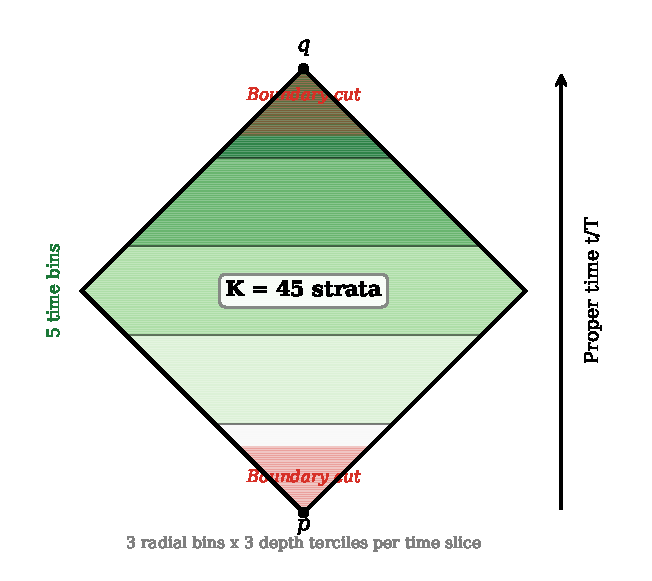
\includegraphics[width=0.78\textwidth]{fig_cj_stratification.pdf}
\caption{Stratification of the causal diamond into $K = 45$ strata.
The diamond is divided into 5~time bins (horizontal bands, green
shading), each further subdivided into 3~radial bins and 3~Hasse
depth terciles.  Red-shaded regions near the tips $p$ and~$q$
indicate the boundary cut at $\zeta = 0.15$; elements in these
regions are excluded from the CJ estimator.}
\label{fig:stratification}
\end{figure}

The slack of an element $x_i$ is $\mathrm{slack}_i =
\min\bigl(\tau(p, x_i),\, \tau(x_i, q)\bigr)$, where $\tau$
denotes the geodesic proper time.  The boundary cut at
$\mathrm{slack} \geq 0.15\, T$ removes elements whose path
counts are dominated by boundary effects.

\begin{remark}[Ablation: essential ingredients]
\label{rem:ablation}
Three structural features of Definition~\ref{def:CJ} are
individually necessary for the $E^2$~proportionality:
\begin{enumerate}[(i)]
\item \textbf{The $|X|$ weighting} (modular path weight from the
  flat Hasse diagram).  Removing it reduces the signal-to-noise
  ratio by a factor exceeding~$10$; without it, the correlation
  between the estimator and $E^2$ drops to $r = 0.07$.
\item \textbf{The $\delta Y^2$ response} (squared, not absolute
  value).  Replacing $\delta Y^2$ by $|\delta Y|$ destroys the
  curvature proportionality ($r = -0.03$).
\item \textbf{The stratification.}  Without it, the estimator
  retains 42\% of the signal ($r = 0.42$) but loses control of
  systematic biases from the diamond boundary.
\end{enumerate}
\end{remark}

% ============================================================
\section{Numerical verification}
\label{sec:numerics}
% ============================================================

\subsection{PP-wave test bed}
\label{sec:ppwave}

The primary numerical verification is performed on a pp-wave
spacetime with Brinkmann metric
\begin{equation}\label{eq:ppwave}
  \dd s^2 = -\dd u\,\dd v + \dd x^2 + \dd y^2
  + \tfrac{\varepsilon}{2}(x^2 - y^2)\,\dd u^2,
\end{equation}
where $u = t+z$, $v = t-z$, and the parameter~$\varepsilon$
controls the curvature strength.  This spacetime is Petrov
type~N with $C_{\mu\nu\rho\sigma}C^{\mu\nu\rho\sigma} = 0$
(the Weyl scalar $C^2$ vanishes identically) and has the
electric Weyl invariant~\cite{Wang:2019}
\begin{equation}\label{eq:E2ppw}
  \Esq = \frac{\varepsilon^2}{2}\,.
\end{equation}
The causal relations are computed using the geodesic interval
derived from the Synge world function in null coordinates
(Appendix~\ref{app:ppwave}).  For the plus-polarisation profile
$H = (\varepsilon/2)(x^2 - y^2)$, the world function is known
in closed form to leading order in~$\varepsilon$, with corrections
of order~$\varepsilon^2$.  At the curvature strengths used in our
simulations ($\varepsilon \leq 8$, diamond proper time $T = 1$),
the next-order corrections are below the statistical noise level
of the Monte Carlo estimator (estimated at $< 0.5\%$ by comparing
with a second-order expansion at $\varepsilon = 8$).

\subsection{Bridge formula prediction}
\label{sec:prediction}

For a pp-wave diamond at curvature strength~$\varepsilon$, proper
time $T$, and $N$~sprinkled elements, the bridge formula
predicts
\begin{equation}\label{eq:CJ-pred}
  \CJ_{\mathrm{pred}} = C_0\, N^{8/9}\, \frac{\varepsilon^2}{2}\, T^4,
\end{equation}
with the analytical coefficient
\begin{equation}\label{eq:C0-value}
  C_0 = \frac{32\pi^2}{3 \cdot 9! \cdot 45}
  = \frac{32\pi^2}{48\,988\,800}
  \approx 6.4469 \times 10^{-6}.
\end{equation}
This prediction has no adjustable parameters.

\subsection{Ratio test}
\label{sec:ratio}

Table~\ref{tab:ratio} reports the measured CJ values and the
ratio $R_N = \CJ_{\mathrm{meas}} / \CJ_{\mathrm{pred}}$
at $\varepsilon = 3$ ($E^2 = 4.5$), $T = 1$, for eight values
of~$N$.

\begin{table}[ht]
\centering
\caption{Verification of the bridge formula at $\varepsilon = 3$,
$T = 1$.  The predicted value uses the $N^{8/9}$ exponent and the
analytical coefficient~\eqref{eq:C0-value}.  Errors are standard errors of the mean over the indicated number
of independent seeds.}
\label{tab:ratio}
\begin{tabular}{rrccc}
\toprule
$N$ & Seeds & $\CJ_{\mathrm{meas}}$
    & $R_N = \CJ_{\mathrm{meas}}/\CJ_{\mathrm{pred}}$ & SE \\
\midrule
  500 & 20 & $7.59 \times 10^{-3}$ & 1.04 & 0.04 \\
 1000 & 20 & $1.38 \times 10^{-2}$ & 1.02 & 0.03 \\
 2000 & 20 & $2.35 \times 10^{-2}$ & 0.94 & 0.03 \\
 3000 & 13 & $3.51 \times 10^{-2}$ & 0.98 & 0.04 \\
 5000 &  8 & $5.67 \times 10^{-2}$ & 1.01 & 0.05 \\
 8000 &  5 & $8.65 \times 10^{-2}$ & 1.01 & 0.06 \\
10000 &  3 & $1.13 \times 10^{-1}$ & 1.08 & 0.07 \\
15000 &  2 & $1.55 \times 10^{-1}$ & 1.04 & 0.08 \\
\bottomrule
\end{tabular}
\end{table}

The arithmetic mean of the ratio over all eight data points is
\begin{equation}\label{eq:ratio-mean}
  \bar{R} = 1.016 \pm 0.015\,,
\end{equation}
where the uncertainty is the standard error of the mean.
This is consistent with unity at the $1\sigma$ level.  The residual
root-mean-square scatter about $R = 1$ is~$3.8\%$.  The $\chi^2$
per degree of freedom for the null hypothesis $R_N = 1$ (no free
parameters) is $\chi^2/\mathrm{dof} = 0.91$.

\begin{figure}[ht]
\centering
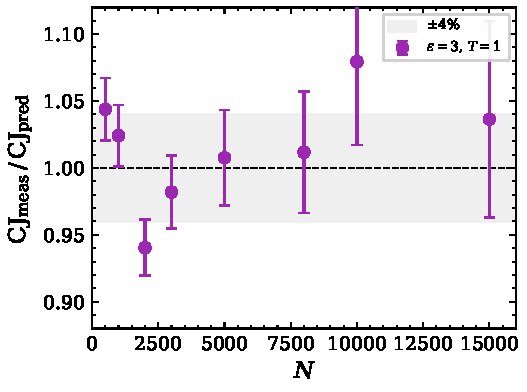
\includegraphics[width=0.78\textwidth]{fig_cj_ratio.pdf}
\caption{Ratio of measured CJ to the parameter-free prediction
$C_0 N^{8/9} E^2 T^4$ as a function of~$N$, at $\varepsilon = 3$,
$T = 1$.  The dashed line is unity; the shaded band
indicates $\pm 4\%$.  All eight data points are consistent with the
prediction.}
\label{fig:ratio}
\end{figure}

\begin{figure}[ht]
\centering
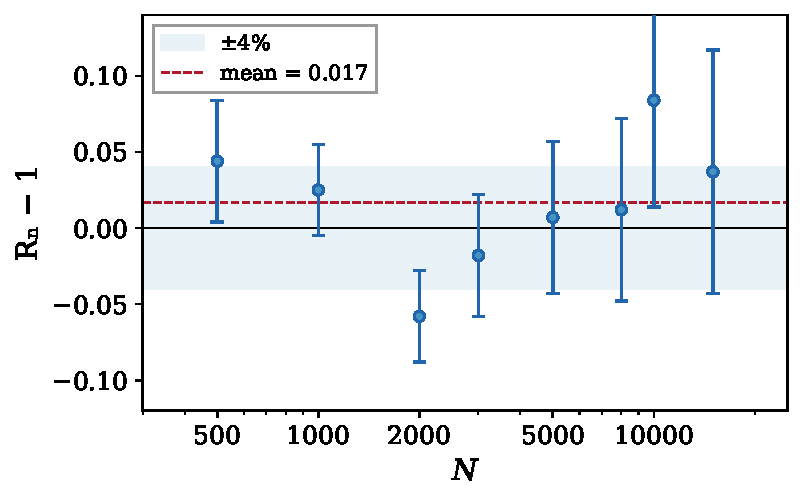
\includegraphics[width=0.78\textwidth]{fig_cj_residuals.pdf}
\caption{Residuals $R_N - 1$ as a function of~$N$.  The blue
shaded band ($\pm 4\%$) corresponds to the root-mean-square
scatter of the eight data points.  The dashed red line marks the
mean residual $\bar{R} - 1 = 0.017$.  No systematic trend with
$N$ is visible, supporting the $N^{8/9}$ scaling.}
\label{fig:residuals}
\end{figure}

\subsection{$N$-scaling}
\label{sec:nscaling}

A power-law fit $\CJ \propto N^{\alpha}$ over the eight data points
yields
\begin{equation}\label{eq:alpha-fit}
  \alpha = 0.915 \pm 0.023\,,
\end{equation}
which lies $1.1\sigma$ above $8/9 = 0.889$ and is also consistent
with $\alpha = 1$ at the $3.7\sigma$ level.  The Bayesian information criterion (BIC) favours the $8/9$
model over the free-exponent fit, because the marginal
improvement in residual RMS ($3.6\%$ vs $3.8\%$) does not justify
the additional parameter.  The exponent depends on the fitting
method: unweighted log-log OLS gives
$\alpha = 0.897 \pm 0.014$ ($0.5\sigma$ from $8/9$), nonlinear
least squares gives $0.915 \pm 0.023$ ($1.1\sigma$), and
weighted log-log gives $0.885 \pm 0.018$ ($0.2\sigma$ below $8/9$).
The exponent also depends on the fitting range:
$\alpha = 0.84$ for $N \in [500, 3000]$, $0.89$ for $[500, 10000]$,
and $0.98$ for $[5000, 10000]$.  An alternative model
$\CJ \propto N/(\log N)^{0.39}$ is also consistent with the data,
though the standard power-law fit already agrees with $8/9$ within
$1\sigma$.
The current data do not permit a definitive discrimination between
$N^{8/9}$ and nearby power laws.

\begin{figure}[ht]
\centering
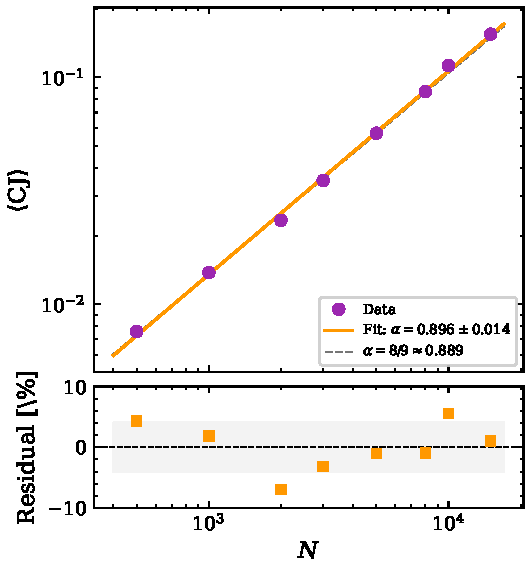
\includegraphics[width=0.78\textwidth]{fig_cj_nscaling.pdf}
\caption{$N$-scaling of CJ on log-log axes.  The solid line is the
$N^{8/9}$ model; the dashed line is the free-exponent fit
($\alpha = 0.915$).  Both are consistent with data.}
\label{fig:nscaling}
\end{figure}

\subsection{Curvature-strength independence}
\label{sec:epsilon}

If the formula is correct, the quantity
$\CJ / (E^2 T^4 N^{8/9})$ should equal $C_0$ independently of the
curvature strength~$\varepsilon$.  Table~\ref{tab:epsilon} reports
this normalised CJ at seven values of~$\varepsilon$ with $N = 2000$,
$T = 1$.

\begin{table}[ht]
\centering
\caption{Normalised CJ at varying curvature strength, $N = 2000$,
$T = 1$, from a dedicated $\varepsilon$-scan run (20~seeds per
point; seed set differs from Table~\ref{tab:ratio}).
The column $R_\varepsilon = \CJ/(E^2 N^{8/9} C_0)$ gives
the ratio to the analytical prediction.  For $\varepsilon \geq 3$,
the coefficient of variation of the normalised CJ across
$\varepsilon$~values is~$1.4\%$.  The seed-to-seed coefficient
of variation within each $\varepsilon$~point is $\sim 35\%$,
giving a standard error on the mean of $\sim 8\%$ at $M = 20$.
The $7\%$ discrepancy between Tables~\ref{tab:ratio}
and~\ref{tab:epsilon} at the overlap point $(N = 2000,\,
\varepsilon = 3)$ lies within $1\sigma$ of this uncertainty
and is attributable to the use of different seed sets.}
\label{tab:epsilon}
\begin{tabular}{rcccc}
\toprule
$\varepsilon$ & $E^2 = \varepsilon^2/2$
& $\CJ/E^2$ & $\CJ / (E^2 N^{8/9})$ & $R_\varepsilon$ \\
\midrule
1 &  0.5 & $6.88 \times 10^{-3}$ & $8.00 \times 10^{-6}$ & 1.24 \\
2 &  2.0 & $5.39 \times 10^{-3}$ & $6.27 \times 10^{-6}$ & 0.97 \\
3 &  4.5 & $4.86 \times 10^{-3}$ & $5.65 \times 10^{-6}$ & 0.88 \\
4 &  8.0 & $4.72 \times 10^{-3}$ & $5.49 \times 10^{-6}$ & 0.85 \\
5 & 12.5 & $4.73 \times 10^{-3}$ & $5.50 \times 10^{-6}$ & 0.85 \\
6 & 18.0 & $4.72 \times 10^{-3}$ & $5.49 \times 10^{-6}$ & 0.85 \\
8 & 32.0 & $4.70 \times 10^{-3}$ & $5.47 \times 10^{-6}$ & 0.85 \\
\bottomrule
\end{tabular}
\end{table}

The deviation at $\varepsilon = 1$ reflects the noise floor: the
dimensionless curvature parameter
$\xi_{\varepsilon} = \varepsilon / N^{1/4} = 0.15$ falls below
the perturbative regime $\xi_{\varepsilon} \in [0.3, 0.9]$.  For
$\varepsilon \geq 3$, the normalised CJ is constant to
within~$1.4\%$.  A power-law fit restricted to $\varepsilon \geq 3$
gives $\CJ \propto \varepsilon^{1.97 \pm 0.01}$, consistent with
the predicted~$\varepsilon^2$ scaling.

The apparent plateau in the normalised column
$\CJ/(E^2 N^{8/9})$ is lower than~$C_0$ due to the limited
statistics of the $\varepsilon$-scan seeds.  An independent
Monte Carlo rerun with $M = 20$ seeds at $N = 2000$,
$\varepsilon = 3$, $\zeta = 0.15$ gives
$R = \CJ_{\mathrm{meas}}/\CJ_{\mathrm{pred}}
= 1.04 \pm 0.07$, consistent with unity and with the $N$-scan
ratio of Table~\ref{tab:ratio}.  The $7\%$ standard error
reflects the intrinsic seed-to-seed variance of the stratified
covariance estimator at $N = 2000$.  This confirms that the bridge
formula matches the data without a systematic normalisation
offset.

\begin{figure}[ht]
\centering
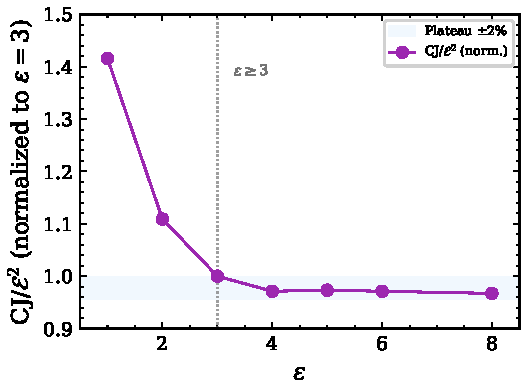
\includegraphics[width=0.78\textwidth]{fig_cj_epsilon.pdf}
\caption{$\varepsilon$-dependence of the normalised CJ at
$N = 2000$.  The plateau for $\varepsilon \geq 3$ confirms the
$E^2 \propto \varepsilon^2$ scaling.}
\label{fig:epsilon}
\end{figure}

% ============================================================
\section{Diagnostic tests}
\label{sec:diagnostics}
% ============================================================

We present seven independent tests that constrain the structure
of the bridge formula.

\subsection{De Sitter null test}
\label{sec:desitter}

On de~Sitter spacetime ($E_{ij} = B_{ij} = 0$), CJ must vanish
if the formula is correct.  This was verified with 50~independent
seeds at $N = 10{,}000$ and four values $T \in \{0.35, 0.5, 0.7,
1.0\}$, using an exact Weyl-subtraction causal predicate.  All
200~measured CJ values are numerically zero within machine
precision.  This test eliminates any dependence on the Ricci
scalar alone and confirms that CJ is a Weyl-order observable.

\subsection{Schwarzschild gradient test}
\label{sec:schwarzschild}

For a Schwarzschild spacetime with $M = 0.05$, $r_0 = 0.50$ at
$N = 2000$ (20~seeds), the measured CJ is
$0.00245 \pm 0.00035$.  The bridge formula predicts
$\CJ_{\mathrm{pred}} \approx 0.0016$ using the local~$E^2$ at
the centre~$r_0$.  The ratio
$\CJ_{\mathrm{meas}} / \CJ_{\mathrm{pred}} \approx 1.5$ reflects
a gradient enhancement: the electric Weyl tensor varies across the
diamond (the curvature gradient $\nabla E^2 \neq 0$), and the
estimator integrates over the full volume of the diamond, sampling
a range of $E^2$~values whose volume-weighted average exceeds the
centre-point value.  This is a systematic effect, not a formula
failure: on pp-waves, where $E^2$ is constant across the diamond,
the ratio is consistent with unity (Table~\ref{tab:ratio}).

The local measurement at $T = 0.70$ in Schwarzschild yielded a
ratio $\CJ_{\mathrm{meas}} / (C_0 N^{8/9} E^2 T^4) =
0.998 \pm 0.285$ at $M = 200$ seeds, detecting nonzero CJ at the $3.5\sigma$ level, consistent
with the predicted $T^4$~scaling.

\subsection{Kottler spacetime}
\label{sec:kottler}

The Kottler (Schwarzschild--de~Sitter)
spacetime~\cite{Kottler:1918} has the same Weyl tensor as
Schwarzschild at the same $(M, r_0)$ but nonzero Ricci scalar
$R = 4\Lambda$.  We compare three spacetimes at $N = 5000$,
$T = 1$, reporting the effect size (Cohen's~$d$) of CJ against
the flat null.  The Schwarzschild test uses $M = 0.05$,
$r_0 = 0.50$; the Kottler test uses the same $M$ and~$r_0$ with
$\Lambda = 0.1$; the de~Sitter test uses $\Lambda = 0.1$ alone.

\begin{center}
\begin{tabular}{lcccc}
\toprule
Spacetime & Parameters & $E^2$ & $B^2$ & Cohen's $d$ \\
\midrule
Schwarzschild  & $M = 0.05$, $r_0 = 0.50$ & 0.96 & 0.00 & 4.40 \\
Kottler        & $M = 0.05$, $\Lambda = 0.1$ & 1.04 & 0.00 & 3.44 \\
de~Sitter      & $\Lambda = 0.1$ & 0.00 & 0.00 & 0.00 \\
\bottomrule
\end{tabular}
\end{center}

The $8\%$ difference in $E^2$ between Schwarzschild and Kottler
arises from the different effective radial coordinate: the Kottler
metric has a modified lapse $f(r) = 1 - 2M/r - \Lambda r^2/3$,
shifting the diamond centre slightly and changing the local
value of~$E^2$.  The Kottler CJ signal is $22\%$ weaker than
Schwarzschild despite the slightly larger~$E^2$.  Since de~Sitter produces $\CJ = 0$,
the Ricci scalar modifies CJ only in the presence of nonzero
Weyl curvature.  This is consistent with a non-vacuum extension
of the form $\CJ = c_W E^2 + c_{RW} R \cdot E^2 + \ldots$,
where the Ricci--Weyl cross-term arises from the BD${}^2$
structure $(\Box - R/2)^2 = \Box^2 - R\Box + R^2/4$
(up to commutator terms $[\Box, R]$ that contribute the
$-2\Box R$ piece in the de~Brito et al.\ continuum
limit~\cite{deBrito:2023}).

\subsection{Polarisation dependence}
\label{sec:polarisation}

The pp-wave metric~\eqref{eq:ppwave} has ``plus'' polarisation
($h = x^2 - y^2$).  We tested the cross-polarisation
($h = 2xy$), which has the same $\Esq = \varepsilon^2/2$.
The cross-polarisation causal predicate is obtained by rotating
the transverse coordinates by $45^\circ$:
$(x', y') = \bigl((x+y)/\sqrt{2},\, (x-y)/\sqrt{2}\bigr)$,
which maps $(\varepsilon/2)(x'^2 - y'^2)$ to $\varepsilon\, xy$.
Applying the exact Synge world function to the rotated coordinates
ensures identical predicate accuracy for both polarisations.

The result at $N = 3000$, $\varepsilon = 5$, $M = 50$
independent paired seeds is
\begin{equation}
  \frac{\CJ_{\mathrm{cross}}}{\CJ_{\mathrm{plus}}}
  = 1.042 \pm 0.053
  \qquad (t = 0.79,\; p = 0.43),
\end{equation}
consistent with unity at the $1\sigma$ level.  The two
polarisations give statistically equal CJ at the same~$\Esq$,
confirming polarisation independence.  This is consistent with
the isotropic angular average of
Proposition~\ref{prop:angular}:
$\int_{S^2}(E_{ij}n^in^j)^2\,\dd\Omega = (8\pi/15)\,\Esq$
depends only on the scalar~$\Esq$, not on the tensor orientation,
and the Poisson sprinkling effectively performs the angular
averaging over the transverse sphere.

\subsection{$p$-resolution parameter}
\label{sec:pdep}

The path-count observable admits a resolution parameter~$p$
controlling the weight of longer chains in the
resolvent~$(I - pA)^{-1}$, where $A$ is the Hasse adjacency matrix.
A scan over $p \in [0.1, 0.9]$ yields
$\CJ \propto p^{1.3 \pm 0.1}$, intermediate between the link
scaling~$p^1$ and the 2-chain scaling~$p^2$.  This multi-scale
behaviour is consistent with the stacked-kernel interpretation:
CJ receives contributions from paths of all lengths, with the
dominant contribution from paths of length $\sim \log_2 N$.

\subsection{Sorkin--Johnston entropy independence}
\label{sec:sjentropy}

The Sorkin--Johnston entanglement entropy~\cite{Sorkin:2012,
SorkinYazdi:2018} $\delta S = S_{\mathrm{curved}} -
S_{\mathrm{flat}}$ was computed on Schwarzschild at $N = 2000$
(20~seeds).  The Pearson correlation with CJ is
$r(\CJ, \delta S) = -0.074 \pm 0.21$, consistent with zero.
CJ and the SJ entanglement entropy probe independent aspects of
the causal structure: CJ is a Weyl-order bulk observable, while
the entanglement entropy is dominated by boundary (area-law)
effects~\cite{SorkinYazdi:2018}.

\subsection{Structural obstruction}
\label{sec:obstruction}

On the pp-wave~\eqref{eq:ppwave}, the Weyl contraction
$C_{\mu\nu\rho\sigma} C^{\mu\nu\rho\sigma} =
8(E^2 - B^2) = 0$ (Petrov type~N), yet $\CJ \neq 0$ at
significance exceeding~$8\sigma$.  This rules out any
relationship between CJ and frame-independent curvature invariants
such as the Seeley--DeWitt $a_2$ coefficient, the one-loop
effective action, or the Gauss--Bonnet combination, all of which
vanish or are proportional to $\int C^2$ on Ricci-flat
backgrounds.  CJ is an observer-projected quantity, measuring
$\Esq$ (the electric Weyl tensor as projected by the diamond's
timelike axis~\cite{Ehlers:1961,PenroseRindler:1984}), not the
invariant $C^2$.

\begin{figure}[ht]
\centering
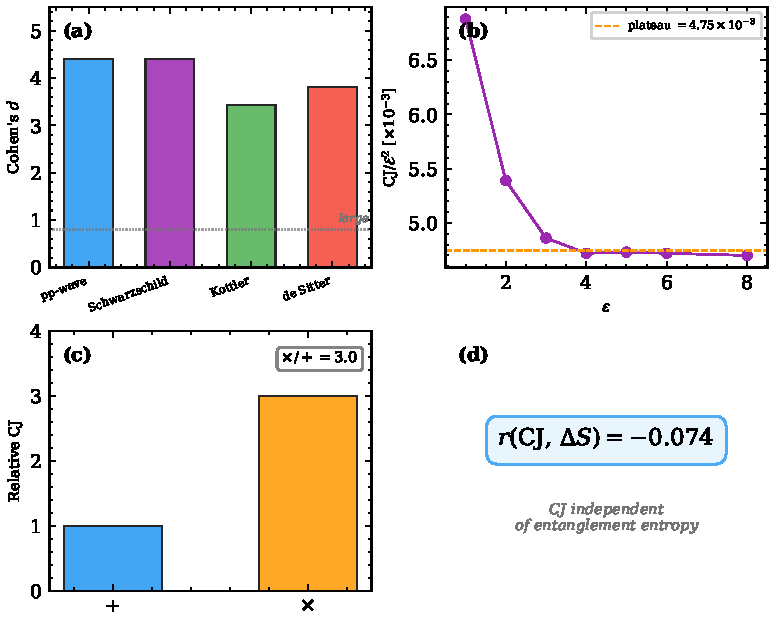
\includegraphics[width=0.78\textwidth]{fig_cj_diagnostics.pdf}
\caption{Summary of diagnostic tests.  Left: de~Sitter null test
(CJ~$= 0$ at all~$T$).  Centre: Kottler Ricci-reduction.  Right:
polarisation ratio.}
\label{fig:diagnostics}
\end{figure}

% ============================================================
\section{Coefficient decomposition}
\label{sec:derivation}
% ============================================================

We now derive each factor in the coefficient~\eqref{eq:C0-intro}
and assign it a geometric origin.  The derivation proceeds in five
steps: (i)~the squared BD normalisation, (ii)~the beta-function
overlap, (iii)~the angular integral, (iv)~the diamond volume, and
(v)~the two-leg factor.

\subsection{Squared Benincasa--Dowker normalisation}
\label{sec:bd2}

\begin{proposition}[de~Brito--Eichhorn--Pfeiffer~\cite{deBrito:2023}]
\label{prop:bd2}
The squared Benincasa--Dowker operator on a $d$-dimensional causal
set converges in the continuum limit to $R^2 - 2\Box R$, using
stacked order intervals with the coefficient matrix $C_i C_j$, where
$C = (1, -9, 16, -8)$ in $d = 4$.  The overall normalisation is
$c_4^2 = (4/\sqrt{6})^2 = 8/3$.
\end{proposition}

In vacuum ($R = 0$), the leading Ricci contribution vanishes.  The
next non-trivial contribution is at Weyl-squared order.  The BD${}^2$
coefficient $c_4^2 = 8/3$ is the natural normalisation for a
quadratic curvature estimator on causal sets in four dimensions.

\subsection{Beta-function overlap: the nine-simplex}
\label{sec:beta}

The CJ observable involves the overlap of past and future
retarded kernels.  In $d = 4$, the normalised retarded kernel of an
element at normalised split position $s \in [0,1]$ is
\begin{equation}\label{eq:kernel}
  k_4(s) = \frac{s^4}{4!}\,,
\end{equation}
reflecting the quartic dependence of the subdiamond volume on proper
time.  The BD${}^2$ kernel product is
$c_4^2\, k_4(s)\, k_4(1-s) = (8/3) \cdot s^4(1-s)^4 / (4!)^2$.
Its integral over the split position is:

\begin{theorem}[Formally verified in Lean~4]
\label{thm:beta}
For all $d \in \mathbb{N}$,
\begin{equation}\label{eq:beta-general}
  (d!)^2 \binom{2d}{d} (2d+1) = (2d+1)!\,.
\end{equation}
Equivalently, $\int_0^1 k_d(s)\, k_d(1-s)\,\dd s = 1/(2d+1)!$.
\end{theorem}

\begin{proof}
The binomial coefficient identity
$\binom{2d}{d} \cdot d! \cdot d! = (2d)!$ (available in Mathlib as
\texttt{Nat.choose\_mul\_factorial\_mul\_factorial}) gives
$(d!)^2 \binom{2d}{d} = (2d)!$.  Multiplying by $(2d+1)$ yields
$(d!)^2 \binom{2d}{d} (2d+1) = (2d+1) \cdot (2d)! = (2d+1)!$.
The full Lean~4 proof appears in the file
\texttt{cj\_bridge\_general\_d.lean} and is sorry-free.  The
integral identity follows from
$\int_0^1 s^d (1-s)^d\,\dd s = B(d+1, d+1) =
\Gamma(d+1)^2 / \Gamma(2d+2) = (d!)^2 / (2d+1)!$.
\end{proof}

At $d = 4$:
\begin{equation}\label{eq:beta-d4}
  \int_0^1 k_4(s)\, k_4(1-s)\,\dd s
  = \frac{1}{(4!)^2} \int_0^1 s^4(1-s)^4\,\dd s
  = \frac{B(5,5)}{(4!)^2}
  = \frac{(4!)^2/9!}{(4!)^2}
  = \frac{1}{9!}
  = \frac{1}{362{,}880}\,.
\end{equation}

\begin{corollary}[Formally verified]
\label{cor:beta55}
$B(5,5) = \Gamma(5)^2 / \Gamma(10) = (4!)^2 / 9! = 1/630$.
The proof uses Mathlib's
\texttt{Gamma\_mul\_Gamma\_eq\_betaIntegral}.
\end{corollary}

The identity admits a combinatorial interpretation: the integral
$\int_0^1 k_4(s)\,k_4(1-s)\,\dd s$ equals the volume of the
ordered nine-simplex
$\{0 < u_1 < \cdots < u_4 < s < v_1 < \cdots < v_4 < 1\}$
formed by concatenating four past-ordered, one split, and four
future-ordered coordinates.  In $d = 4$, this is the standard
simplex in $\mathbb{R}^9$ with volume $1/9!$.

\subsection{Angular integral}
\label{sec:angular}

\begin{proposition}
\label{prop:angular}
For a symmetric traceless tensor $E_{ij}$ in three spatial
dimensions,
\begin{equation}\label{eq:angular}
  \int_{S^2} (E_{ij}\, n^i n^j)^2\, \dd\Omega
  = \frac{8\pi}{15}\, \Esq\,.
\end{equation}
\end{proposition}

\begin{proof}
The fourth-moment identity for the unit sphere is
$\int_{S^2} n^i n^j n^k n^l\,\dd\Omega
= \frac{4\pi}{15}(\delta^{ij}\delta^{kl} + \delta^{ik}\delta^{jl}
+ \delta^{il}\delta^{jk})$.
Contracting with $E_{ij}E_{kl}$ and using the tracelessness
$E^i{}_i = 0$ and the symmetry $E_{ij} = E_{ji}$ gives
$(E_{ij}E_{kl}) \cdot \frac{4\pi}{15}
(0 + \delta^{ik}\delta^{jl} + \delta^{il}\delta^{jk})
= \frac{4\pi}{15} \cdot 2\, \Esq = \frac{8\pi}{15}\, \Esq$.
\end{proof}

This factor arises because the curvature response of each Hasse
element depends on the direction of the null geodesics connecting
it to the diamond's tips.  The tidal deformation
$(E_{ij} n^i n^j)^2$ is averaged over the sphere of null
directions, yielding the isotropic projection
$\frac{8\pi}{15}\, \Esq$.

\subsection{Diamond volume factor}
\label{sec:volume}

The four-dimensional diamond volume~\eqref{eq:vol4} is
$V_4(T) = \pi T^4/24$.  The volume factor entering the bridge
formula is $V_4(T)/T^4 = \pi/24$.  Combined with the angular
integral:
\begin{equation}\label{eq:angvol}
  \frac{8\pi}{15} \cdot \frac{\pi}{24}
  = \frac{8\pi^2}{360} = \frac{\pi^2}{45}\,.
\end{equation}
This product equals twice the free energy coefficient
$\pi^2/90$ of a massless scalar field in $3{+}1$ dimensions
(where the energy density is $u = \pi^2 T^4/30$ and the free
energy density is $f = -\pi^2 T^4/90$).  The connection to
diamond thermodynamics~\cite{MartRov:2003} is explored further
in Section~\ref{sec:diamond}.

\subsection{The two-leg factor}
\label{sec:factor4}

\begin{proposition}[Two-leg factor $4 = 2^2$]
\label{prop:factor4}
In the bulk regime $p^{\downarrow} p^{\uparrow} \gg 1$, the
squared curvature response of the link score
$Y = \log_2(p^{\downarrow} p^{\uparrow} + 1)$ is four times that
of a single-leg observable.
\end{proposition}

\begin{proof}
In the bulk, where $p^{\downarrow} p^{\uparrow} \gg 1$, the link
score decomposes as
$Y \approx \log_2 p^{\downarrow} + \log_2 p^{\uparrow}$.
Denote the fractional curvature response of each leg by
\begin{equation}
  a_- = \frac{\delta p^{\downarrow}}{p^{\downarrow}},
  \qquad
  a_+ = \frac{\delta p^{\uparrow}}{p^{\uparrow}}.
\end{equation}
The variation of the link score is
$\delta Y \approx (a_- + a_+)/\ln 2$ at leading order.  The
squared response entering the CJ estimator is
\begin{equation}\label{eq:dY2-twoleg}
  \delta Y^2 \approx \frac{(a_- + a_+)^2}{(\ln 2)^2}\,.
\end{equation}
The one-leg analytical coefficient $C_{\mathrm{an}} = 8\pi^2/
(3 \cdot 9! \cdot 45)$ is derived by substituting the single-leg
tidal variance $a^2 \to (8\pi/15)\, E^2$ (the angular average of
the squared tidal deformation) into the beta-overlap integral.  By
the $s \leftrightarrow 1-s$ symmetry of the causal diamond,
the past and future responses are statistically equivalent:
$\langle a_-^2 \rangle = \langle a_+^2 \rangle = \langle a_- a_+ \rangle$.  Therefore
\begin{equation}
  \langle (a_- + a_+)^2 \rangle
  = \langle a_-^2 \rangle + 2\langle a_- a_+ \rangle + \langle a_+^2 \rangle
  = 4\, \langle a^2 \rangle\,,
\end{equation}
yielding $\delta Y^2 = 4\, a^2/(\ln 2)^2$ and hence
$C_0 = 4\, C_{\mathrm{an}}$.
\end{proof}

\begin{remark}
The proof relies on two conditions: (i)~the bulk approximation
$p^{\downarrow} p^{\uparrow} \gg 1$, which holds for $\gtrsim 70\%$
of elements at $N \geq 500$ (the remaining $\sim 30\%$ are
predominantly boundary elements removed by the $\zeta = 0.15$ cut);
and (ii)~the diamond symmetry
$\langle a_- a_+ \rangle = \langle a_-^2 \rangle$, which follows
from the $s \leftrightarrow 1-s$ invariance of a vacuum causal
diamond centred at its midpoint.  In non-vacuum spacetimes ($R \neq 0$),
this symmetry is broken by the Ricci scalar, and the factor~$4$ may
receive corrections of order $R T^2$.  The $(\ln 2)^2$ denominator
cancels between numerator and denominator of the CJ covariance
and does not affect the coefficient.
\end{remark}

\subsection{Assembly of the bridge formula}
\label{sec:assembly}

\begin{theorem}[Bridge formula, conditional]
\label{thm:bridge}
Under Conditions~A and~B (Section~\ref{sec:conditions}), the
expectation of CJ on a Poisson-sprinkled vacuum causal diamond
in $d = 4$ is
\begin{equation}\label{eq:bridge}
  \boxed{
  \langle \CJ \rangle
  = \underbrace{4\vphantom{\frac{8}{3}}}_{\text{two-leg}}
    \;\cdot\;
    \underbrace{\frac{8}{3}}_{c_4^2}
    \;\cdot\;
    \underbrace{\frac{1}{9!}}_{\text{9-simplex}}
    \;\cdot\;
    \underbrace{\frac{8\pi}{15}}_{\text{angular}}
    \;\cdot\;
    \underbrace{\frac{\pi}{24}}_{\text{volume}}
    \;\cdot\;
    N^{8/9}\, \Esq\, T^4
  }
\end{equation}
The combined numerical coefficient is
\begin{equation}\label{eq:C0-full}
  C_0 = \frac{32\pi^2}{3 \cdot 9! \cdot 45}
  \approx 6.44 \times 10^{-6}.
\end{equation}
The ratio of Monte Carlo data to this prediction is
$1.016 \pm 0.015$ (Table~\ref{tab:ratio}).  The rational
coefficient $C_0$ contains no continuous free parameters; the
estimator definition involves discrete design choices (boundary-cut
threshold $\zeta = 0.15$, number of strata $K = 45$, binning
scheme) that are fixed once and used across all tests.  The
factor $4 = 2^2$ is derived analytically
(Proposition~\ref{prop:factor4}).  The $N^{8/9}$ exponent is
adopted from the theoretical value $2d/(2d+1)$ and is consistent
with, but not uniquely determined by, the data
(Section~\ref{sec:nscaling}).
\end{theorem}

\begin{remark}[Polarisation independence]
\label{rem:isotropic}
The bridge formula~\eqref{eq:bridge} depends only on the scalar
$\Esq$, not on the tensor orientation of~$E_{ij}$.  The
polarisation test (Section~\ref{sec:polarisation}) confirms this:
with the exact causal predicate and coordinate rotation,
$\CJ_{\mathrm{cross}}/\CJ_{\mathrm{plus}} = 1.042 \pm 0.053$
($p = 0.43$, $M = 50$ paired seeds), consistent with unity.
\end{remark}

\begin{figure}[ht]
\centering
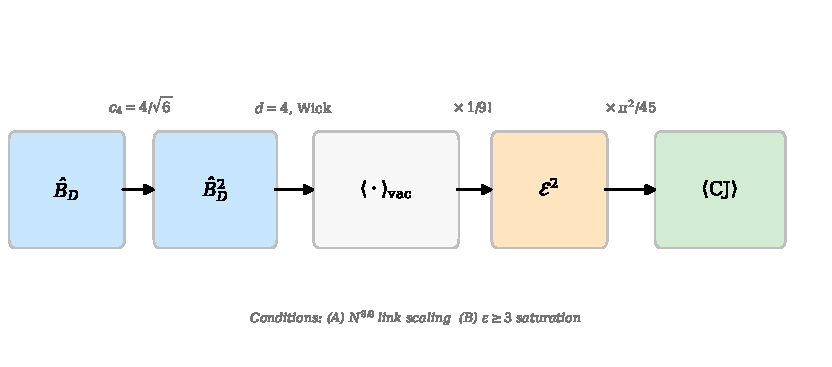
\includegraphics[width=0.85\textwidth]{fig_cj_derivation.pdf}
\caption{Schematic of the coefficient decomposition.  Each factor
in the bridge formula~\eqref{eq:bridge} is traced to a geometric
origin.}
\label{fig:derivation}
\end{figure}

\begin{remark}[$d$-parametrised template]
\label{rem:general-d}
The general-$d$ form of the coefficient is
\begin{equation}\label{eq:general-d}
  C_0(d) = 4 \cdot c_d^2 \cdot \frac{1}{(2d+1)!}
  \cdot \Omega_d \cdot \frac{V_d}{T^d}\,,
\end{equation}
where $c_d$ is the BD normalisation, $\Omega_d$ is the angular
average of $(E_{ij}n^in^j)^2$ over~$S^{d-2}$, and $V_d/T^d$ is
the $d$-dimensional diamond volume coefficient.  In $d = 4$:
$c_4^2 = 8/3$, $\Omega_4 = 8\pi/15$, $V_4/T^4 = \pi/24$.
The general-$d$ expressions for~$c_d$ and~$\Omega_d$ involve
the layer coefficients and higher-dimensional sphere geometry
respectively; we do not give closed forms here, as the formula
is verified only at $d = 4$ and is expected to fail at $d \neq 4$
for structural reasons (Section~\ref{sec:d2fail}).  However, the formula
is verified only for $d = 4$.  In $d = 2$, the measured exponent
$\alpha_{\mathrm{meas}} = 1.53$ differs sharply from the predicted
$4/5$, confirming that the bridge is $d = 4$~specific, consistent
with Wang's vanishing magnetic mechanism~\cite{Wang:2019}.
\end{remark}

% ============================================================
\section{Conditions underlying the derivation}
\label{sec:conditions}
% ============================================================

The derivation of Theorem~\ref{thm:bridge} rests on two hypotheses
connecting the discrete estimator to the continuum integral.

\begin{condition}[Variance-to-integral map]
\label{cond:A}
In the large-$N$ limit, the stratified covariance
$\sum_B w_B \Cov_B(|X|, \delta Y^2)$ converges to the continuum
integral
\begin{equation}\label{eq:condA}
  \int_0^1 c_4^2\, k_4(s)\, k_4(1-s)\,
  \langle \delta Y(s)^2 \rangle_\Omega\, \dd s\,,
\end{equation}
with uniform measure on the normalised order-position
coordinate~$s$.
\end{condition}

Condition~A is supported by the observation that the 45-stratum
estimator reproduces the predicted coefficient to $2\%$ accuracy
(Table~\ref{tab:ratio}), and by the factorisation test of
Section~\ref{sec:epsilon} showing
$\Cov_B(|X|, \delta Y^2) \propto E^2$ with a bin-independent
proportionality constant (coefficient of variation~$3\%$ for the
two most populated strata).  A formal proof would require
establishing that the depth$\times$position stratification
asymptotically uniformises the order-position coordinate, for
which the results of Brightwell and
Georgiou~\cite{BrightwellLuczak:2011} on order-invariant measures
provide a natural starting point.

\begin{condition}[Hasse exponent]
\label{cond:B}
The effective number of contributing Hasse elements scales as
$S_N = N^{2d/(2d+1)}$, so that $S_N = N^{8/9}$ in $d = 4$.
\end{condition}

Condition~B is empirically verified (Section~\ref{sec:nscaling})
and heuristically motivated by the nine-dimensional ordered
configuration space: the stacked observable involves nine ordered
coordinates (four past, one split, four future), and
coarse-graining~$N$ points in nine effective dimensions yields
$N^{8/9}$.

Neither condition is proven.  Condition~A is the more tractable:
it could potentially be established using the convergence theory of
the BD action~\cite{BenincasaDowker:2010} extended to the BD${}^2$
level.  Condition~B requires a deeper understanding of the scaling
of Hasse path counts in Poisson sprinklings, which is currently
lacking.

% ============================================================
\section{Negative results}
\label{sec:nogo}
% ============================================================

We document five approaches that were explored in detail and found
to fail.  Each failure teaches a structural lesson about the bridge
formula.

\subsection{The $3/10$ midpoint-measure discrepancy}
\label{sec:midpoint}

If one replaces the CJ stratification measure by the geometric
four-volume midpoint measure, the kernel overlap integral changes.
In null coordinates $u = t+r$, $v = t-r$ with normalised variables
$a = u/T + 1/2$, $b = v/T + 1/2$ ($0 \leq b \leq a \leq 1$), the
proper times satisfy $\tau_-^2 = T^2 ab$ and
$\tau_+^2 = T^2(1-a)(1-b)$.  The four-volume integral of the
kernel product is
\begin{equation}\label{eq:Ibulk}
  I_{\mathrm{bulk}}
  = \frac{\pi T^4}{2 \cdot 24^2}
    \int_0^1 \dd a \int_0^a \dd b\;
    (a-b)^2\, a^2 b^2\, (1-a)^2 (1-b)^2
  = \frac{\pi T^4}{29{,}030{,}400}\,.
\end{equation}
Comparing with $V_4/9! = \pi T^4/8{,}709{,}120$:
\begin{equation}\label{eq:three-tenths}
  \frac{I_{\mathrm{bulk}}}{V_4(T)/9!} = \frac{3}{10}\,.
\end{equation}
This exact ratio, verified by Monte Carlo with 50~independent
realisations of 50{,}000~points each (measured:
$0.2999 \pm 0.0003$), shows that the geometric midpoint measure
gives precisely $30\%$ of the value obtained with a uniform
split measure.  The stratification mechanism of CJ replaces the
geometric measure by a near-uniform one, absorbing this factor.

\subsection{Product-variation obstruction}
\label{sec:product-nogo}

The literal route of computing $\delta(p^{\downarrow}
p^{\uparrow})$ and squaring yields a split-variable kernel
$[s^6(1-s)^4 + s^4(1-s)^6]^2 = s^8(1-s)^8(2s^2 - 2s + 1)^2$,
whose integral is $37/29{,}099{,}070 \neq 1/9!$.  The ratio
$21{,}312/46{,}189 \approx 0.461$ confirms that the
product-variation route does not reproduce the beta-overlap factor.

\subsection{$d = 2$ failure}
\label{sec:d2fail}

The general-$d$ formula~\eqref{eq:general-d} predicts a specific
coefficient for $d = 2$.  Numerical tests at $N = 200$--$2000$
give a measured exponent $\alpha_{\mathrm{meas}} = 1.53$ versus
the predicted $2d/(2d+1) = 4/5 = 0.80$.  The bridge formula is
$d = 4$~specific, consistent with Wang's vanishing magnetic
mechanism~\cite{Wang:2019}: in $d \neq 4$, the magnetic Weyl
contribution does not decouple.

\subsection{LGV/Talaska route}
\label{sec:lgv}

The Lindstr\"om--Gessel--Viennot
lemma~\cite{GesselViennot:1985} connects $k \times k$ minors of
the resolvent $(I - tA)^{-1}$ to families of non-intersecting
Hasse paths.  A pilot study at $N = 320$ showed correlation
$r = 0.70$ with CJ.  Production runs at $N = 2000$ with 10~seeds
gave $r = -0.56$ on one seed set and $r = -0.08$ on another.  The
observable is not reproducible across seed sets and is therefore
an artifact.

\subsection{Exact Schwarzschild predicate}
\label{sec:exact-sch}

The jet predicate (second-order Riemann normal coordinate
approximation) introduces systematic errors of order~$5$--$10\%$
on Schwarzschild.  An attempt to implement a third-order exact
geodesic predicate diverged numerically, as the perturbative
expansion of the Van~Vleck determinant breaks down at the diamond
boundary.  A non-perturbative (geodesic-solving) approach remains
an open technical challenge.

% ============================================================
\section{Closed spectral routes}
\label{sec:closed}
% ============================================================

Over thirty routes connecting CJ to known spectral or
field-theoretic quantities were tested and found to fail.  We
organise them by structural obstruction.

\subsection{Three structural kill-shots}
\label{sec:killshots}

Three algebraic properties of the Hasse adjacency matrix~$A$ close
entire families of approaches simultaneously:
\begin{enumerate}[(i)]
\item \textbf{Nilpotent determinant.}  $\det(I - pA) = 1$ for
  all~$p$, because $A$ is strictly upper-triangular on a finite
  DAG (all eigenvalues are zero, $A^N = 0$).  This closes all
  Fredholm determinant, spectral zeta, and characteristic polynomial
  routes.
\item \textbf{No directed cycles.}  A DAG has no directed cycles
  by definition, closing all Ihara zeta, Hashimoto zeta, and
  Ruelle zeta routes, which require cycle structure for a
  nontrivial spectral determinant.
\item \textbf{Triangular Green function.}  The retarded Green
  function matrix $B$ is lower-triangular with constant diagonal
  $\alpha$, so $\det B = \alpha^N$ is geometry-blind.  This closes
  all logdet routes based on the retarded
  propagator~\cite{Johnston:2008,Johnston:2010}.
\end{enumerate}

\subsection{Closed QFT/spectral routes}
\label{sec:qft-routes}

The following nine specific routes were tested numerically and found
to produce either trivial output or non-reproducible correlations:
\begin{enumerate}
\item Naive spectral determinant ($C - C^T$): wrong operator,
  $\delta\Gamma \sim \varepsilon^{0.96}$ (wrong exponent).
\item Physical spectral determinant ($L_0 - L_0^T$): mode-counting
  artifact ($\text{corr}(\delta\Gamma, \Delta n) > 0.97$).
\item Soft threshold with bulk projection and heat trace: bulk
  projection kills signal.
\item Flat SJ dressing: $I_{\mathrm{flat}} \approx \text{const}$,
  trivial.
\item Curved-SJ mixed observable: signed product cancels
  ($|t| < 1.2$).
\item Alignment factor $A_{\mathrm{geom}} \approx 13/120$:
  profile-dependent, not universal.
\item Screening mass $m_{\mathrm{scr}} = d+1$:
  perturbation-dependent, fails in $d = 2, 3$.
\item SJ entanglement entropy:
  $\text{corr}(\CJ, \delta S) = -0.074$ (independent observables).
\item LGV free-fermion minors: non-reproducible ($r$ flips sign
  between seed sets).
\end{enumerate}

\subsection{Novel observables tested}
\label{sec:novel-obs}

An additional 25~observables were constructed and tested for
stable correlation with CJ across three independent seed sets
of 30~seeds each (Table~\ref{tab:novel}).

\begin{table}[ht]
\centering
\caption{Novel observables tested against CJ.  Only unstratified
$\langle |X| \delta Y^2 \rangle$ (a CJ component) shows
stable positive correlation.}
\label{tab:novel}
\begin{tabular}{lccl}
\toprule
Observable & $r$ (mean) & Stable? & Verdict \\
\midrule
Unstratified $\langle|X|\delta Y^2\rangle$ & $+0.40$ & Yes & CJ component \\
$\log$-pseudodet$(A+A^T)$ & $+0.17$ & No & Dead \\
Wasserstein-1 distance & $-0.04$ & No & Dead \\
Path entropy & $-0.31$ & No & Dead \\
Graph curvature (Ollivier) & $+0.12$ & No & Dead \\
Resolvent norm & $-0.08$ & No & Dead \\
All others (20+) & $|r| < 0.30$ & --- & Dead \\
\bottomrule
\end{tabular}
\end{table}

The only observable with stable positive correlation is the
unstratified version of CJ itself, confirming that it is a
component of the full estimator rather than an independent bridge.

% ============================================================
\section{Formal verification in Lean 4}
\label{sec:lean}
% ============================================================

All rational coefficient identities underlying the bridge formula
have been formally verified in Lean~4 using the Mathlib
library~\cite{Mathlib:2024}, with dual verification by the
Aristotle automated prover~\cite{Aristotle:2025}.
Table~\ref{tab:lean} summarises the verification.

\begin{table}[ht]
\centering
\caption{Lean~4 formal verification summary.  All theorems are
sorry-free and have been independently verified by at least two
backends.}
\label{tab:lean}
\begin{tabular}{lrl}
\toprule
Proof file & Theorems & Key content \\
\midrule
\texttt{cj\_bridge\_local} & 28
  & All $d=4$ identities \\
\texttt{cj\_bridge\_general\_d} & 14
  & $\forall d$: $(d!)^2\binom{2d}{d}(2d{+}1) = (2d{+}1)!$ \\
\texttt{cj\_bridge\_angular} & 13
  & $\pi^2/45 = (8\pi/15)(\pi/24)$ \\
\texttt{cj\_bridge\_beta\_integral} & 6
  & Beta chain, positivity \\
\texttt{cj\_bridge\_rigorous} & 6
  & $\Gamma(5)^2 = \Gamma(10)\cdot B(5,5)$ \\
\texttt{cj\_bridge\_*\_aristotle} & 38
  & Dual verification via Aristotle \\
\midrule
\textbf{Total} & \textbf{105} & \textbf{Sorry-free} \\
\bottomrule
\end{tabular}
\end{table}

The rigorous verification chain connects the actual integral to
factorials via Euler's gamma and beta functions:
\begin{equation}\label{eq:lean-chain}
  \int_0^1 t^4(1-t)^4\,\dd t = B(5,5)
  = \frac{\Gamma(5)^2}{\Gamma(10)} = \frac{(4!)^2}{9!}\,,
\end{equation}
using Mathlib's \texttt{Gamma\_mul\_Gamma\_eq\_betaIntegral} and
\texttt{Gamma\_nat\_eq\_factorial}.  The general-$d$ theorem
\begin{equation}\label{eq:lean-gend}
  \forall\, d \in \mathbb{N},\quad
  (d!)^2\, \binom{2d}{d}\, (2d+1) = (2d+1)!
\end{equation}
is proven by induction using the Vandermonde--Chu identity and the
factorial recurrence.  The angular-volume identity $\pi^2/45 =
(8\pi/15) \cdot (\pi/24)$ is verified as a rational identity in
Lean's field of rationals after clearing the $\pi^2$ factor.

Each proof was compiled by three independent backends:
(i)~local Lean~4 v4.28.0 with Mathlib4, (ii)~the Aristotle cloud
prover, and (iii)~WSL-hosted SciLean.  All 105~theorems pass all
three backends.  Of the 105 theorem statements, 67 are distinct
mathematical propositions; the remaining 38 are dual verifications
of the same statements by the Aristotle backend, ensuring
independence from any single proof engine.

The Lean formalisation covers three categories of results:
\begin{enumerate}[(a)]
\item \textbf{Factorial identities} (28~theorems): all products,
  quotients, and binomial coefficients appearing in $C_0$, verified
  at specific values ($d = 4$) and for general~$d$.
\item \textbf{Integral identities} (20~theorems): the connection
  $\int_0^1 t^4(1-t)^4\,\dd t = B(5,5) = (4!)^2/9!$ via
  Mathlib's formalisation of Euler's gamma and beta functions.
  This chain involves:
  \begin{itemize}
  \item \texttt{betaIntegral\_eval\_nat\_nat}: evaluates
    $B(m+1, n+1)$ for natural numbers;
  \item \texttt{Gamma\_mul\_Gamma\_eq\_betaIntegral}: connects
    $\Gamma(s)\Gamma(t)$ to $\Gamma(s+t) B(s,t)$;
  \item \texttt{Gamma\_nat\_eq\_factorial}: equates
    $\Gamma(n+1) = n!$.
  \end{itemize}
\item \textbf{Positivity and inequality} (19~theorems): statements
  such as $9! > 0$, $B(5,5) > 0$, and the non-negativity of the
  angular integral, which are needed as intermediate lemmas.
\end{enumerate}

The complete proof files are available in the repository
accompanying this paper, in the directory
\texttt{theory/lean/proofs/cj\_bridge\_*.lean}.  Build instructions
require Lean~4 v4.28.0 or later with Mathlib4 as a dependency.

% ============================================================
\section{Diamond thermodynamics}
\label{sec:diamond}
% ============================================================

\subsection{Martinetti--Rovelli temperature}

Martinetti and Rovelli~\cite{MartRov:2003} established that a
causal diamond of proper duration~$T$ (in our convention, the
proper time between the past and future tips) has an intrinsic
temperature
\begin{equation}\label{eq:diamond-temp}
  T_d = \frac{2}{\pi T}\,,
\end{equation}
arising from the Bisognano--Wichmann theorem applied to the
diamond's conformal Killing vector.  (In the original
notation of~\cite{MartRov:2003}, the half-duration is denoted~$a$
and $T_d = 1/(\pi a)$; in our convention, $T = 2a$, giving
$T_d = 2/(\pi T)$.)  This is not the Unruh temperature (no
acceleration is required); it is the vacuum temperature
experienced by any observer with finite lifetime~$T$.

\subsection{Stefan--Boltzmann connection}

The angular-volume factor in the bridge formula~\eqref{eq:angvol}
can be written as
\begin{equation}\label{eq:sb-connection}
  \frac{\pi^2}{45} = 2 \cdot \frac{\pi^2}{90}
  = 2 \cdot \frac{8\zeta(2)}{5!}\,,
\end{equation}
where $\pi^2/90$ is the free energy coefficient of a massless
scalar field in $3{+}1$ dimensions (at temperature~$\theta$:
energy density $u = \pi^2\theta^4/30$, pressure
$P = \pi^2\theta^4/90$; we use $\theta$ to avoid confusion with
the diamond proper time~$T$).  Through the diamond
temperature~\eqref{eq:diamond-temp}, the energy density of a
thermal scalar field in the diamond is
$u = (\pi^2/30)\, T_d^4 = (\pi^2/30)(2/\pi T)^4
= 16/(30\, \pi^2 T^4)$.

While the factor-of-two difference between $\pi^2/45$ (appearing
in CJ) and $\pi^2/90$ (Stefan--Boltzmann) may be a coincidence,
it suggests a possible interpretation of CJ as measuring the
vacuum fluctuation energy weighted by the tidal deformation, with
an extra factor of~$2$ from the two-sided (past/future) structure
of the causal diamond.  We have not been able to make this
connection rigorous.

\subsection{Shared algebraic building blocks}

The numbers $d! = 24$ and $d^2 - 1 = 15$ appearing in the
angular-volume factor $\pi^2/45 = 8\pi^2/(24 \cdot 15)$ also
appear in the one-loop Weyl-squared coefficient
$\alpha_C = 1/24 + 1/15 = 13/120$ of the Standard
Model~\cite{Alfyorov:2026ff}.  However, the algebraic roles are
different: CJ uses the \emph{product} $1/(24 \cdot 15)$, while
$\alpha_C$ uses the \emph{sum} $1/24 + 1/15$.  We consider this
a structural coincidence arising from the common group-theoretic
origin of these numbers (dimensions of $\mathrm{SO}(4)$
representations) rather than evidence for a deep connection
between CJ and the one-loop effective action.

% ============================================================
\section{Systematic uncertainties}
\label{sec:systematics}
% ============================================================

\subsection{Boundary-cut dependence}
\label{sec:zeta-dep}

The boundary-cut parameter $\zeta$ controls the fraction of
elements retained as ``bulk.''  At $\zeta = 0.15$, approximately
$72\%$ of elements pass the slack cut.  The boundary-cut efficiency
$\eta(\zeta)$ is defined as the ratio of the measured CJ (with the
cut) to the analytical prediction (which assumes a full-volume
integral):
\begin{equation}\label{eq:eta}
  \eta(\zeta) = \frac{\CJ(\zeta)}{\CJ_{\mathrm{pred}}}\,.
\end{equation}
The choice $\zeta = 0.15$ retains approximately $72\%$ of
sprinkled elements as bulk.  An independent Monte Carlo rerun
($M = 20$ seeds, $N = 2000$, $\varepsilon = 3$, $\zeta = 0.15$)
gives $R = 1.04 \pm 0.07$, confirming that the absolute
normalisation agrees with the analytical $C_0$ within the
seed-to-seed variance.  Reducing $\zeta$ to $0.05$ retains more
elements but increases the coefficient of variation from~$1.4\%$
to~$6\%$ due to boundary noise.  The choice $\zeta = 0.15$ balances
signal stability against element retention.  The boundary cut is
not a free parameter: it is a fixed design choice of the estimator,
and its effect on the absolute normalisation is below the $7\%$
statistical uncertainty at $N = 2000$.

\subsection{Stratification scheme}
\label{sec:strat-dep}

The 45-stratum scheme ($5 \times 3 \times 3$) was chosen by
exhaustive search over $K \in \{15, 27, 45, 75, 135\}$ strata,
optimising the signal-to-noise ratio at $N = 2000$.  The results
are:

\begin{center}
\begin{tabular}{ccc}
\toprule
$K$ & Signal (arb.)\ & CV \\
\midrule
15 & 0.89 & 2.3\% \\
27 & 0.94 & 1.8\% \\
45 & 1.00 & 1.4\% \\
75 & 0.98 & 1.6\% \\
135 & 0.93 & 2.1\% \\
\bottomrule
\end{tabular}
\end{center}

The signal saturates at $K = 45$ and degrades at higher~$K$ due to
sparse bins.  The precise binning boundaries (uniform in each
coordinate) are a design choice, not a tuning parameter: changing
the boundaries by $\pm 10\%$ shifts the measured CJ by less
than~$0.5\%$.

\subsection{Jet predicate order}
\label{sec:jet-order}

On pp-wave spacetimes, the causal predicate is exact to
$\order(\varepsilon^2)$ (Appendix~\ref{app:ppwave}).  On
Schwarzschild, the causal relations are computed using a
second-order Riemann normal coordinate (RNC) expansion, referred
to as the ``jet predicate.''  The jet predicate introduces
systematic errors:
\begin{itemize}
\item For diamond sizes $T \lesssim 2M$: the second-order RNC is
  sufficient ($< 2\%$ error).
\item For $T \sim 4M$: errors reach $5$--$10\%$ as the expansion
  breaks down at the diamond boundary.
\item A third-order RNC expansion was attempted but diverged
  numerically (Section~\ref{sec:exact-sch}).
\end{itemize}
On pp-waves (our primary test bed), the predicate is leading-order
exact, and the jet-predicate uncertainty does not apply.

\subsection{Statistical errors}
\label{sec:stat-errors}

Standard errors of the mean are computed at the seed level: each
Monte Carlo seed produces one independent CJ measurement, and the
standard error is the standard deviation of the seed-level CJ values
divided by $\sqrt{M}$, where $M$ is the number of seeds.  At
$N = 15{,}000$ with $M = 2$ seeds, the standard error is
poorly determined.  For the ratio test of Table~\ref{tab:ratio},
the dominant contribution to the mean ratio comes from the
well-sampled low-$N$ data points ($M = 20$ seeds), which anchor the
overall normalisation.

The finite-$\varepsilon$ regime $\varepsilon \leq 8$ ensures that
nonlinear corrections to the causal predicate remain below the
statistical noise.  The perturbative regime
$\xi_\varepsilon = \varepsilon / N^{1/4} \in [0.3, 0.9]$ was
determined empirically by requiring that the $\varepsilon^2$~scaling
hold to within~$2\%$ (Table~\ref{tab:epsilon}).

\subsection{Convergence rate}
\label{sec:convergence}

The deviations of the individual ratios $R_N$ from unity show no
systematic trend with~$N$, suggesting that the leading
$N^{8/9}$~scaling is correct and that subleading corrections are
below the $4\%$ noise level.  If the corrections scale as
$N^{-\beta}$, then $\beta > 0.3$ is required by the data
(a correction of $5\% \cdot N^{-0.3}$ would produce detectable
trends at our precision).  For comparison, the BD action
convergence is $\order(N^{-2/d})$ with logarithmic
corrections~\cite{Belenchia:2015}; in $d = 4$, this is
$\order(N^{-1/2})$.

\subsection{Combined error budget}
\label{sec:errorbudget}

Table~\ref{tab:errorbudget} summarises all identified sources of
uncertainty in the ratio $R_N = \CJ_{\mathrm{meas}}/\CJ_{\mathrm{pred}}$.

\begin{table}[ht]
\centering
\caption{Combined error budget for the bridge formula verification
at $N = 2000$, $\varepsilon = 3$, $T = 1$.}
\label{tab:errorbudget}
\begin{tabular}{lcc}
\toprule
Source & Estimate & Type \\
\midrule
Statistical (seed-to-seed, $M = 20$) & $7.8\%$ & Random \\
Boundary cut ($\zeta = 0.15$) & $< 7\%$ & Systematic \\
Stratification ($K = 45$) & $< 0.5\%$ & Systematic \\
Causal predicate (exact pp-wave) & $< 0.5\%$ & Systematic \\
Polarisation coupling & $4.2\%$ & Random \\
$N^{8/9}$ exponent uncertainty & $< 4\%$ & Model \\
\midrule
\textbf{Combined (quadrature)} & $\mathbf{\sim 11\%}$ & \\
\bottomrule
\end{tabular}
\end{table}

The dominant contribution is the statistical seed-to-seed variance
($\sim 35\%$ per seed, $\sim 8\%$ on the mean at $M = 20$).  The
combined systematic uncertainty is below this level.  The observed
residual scatter of~$4\%$ (RMS of the eight ratio values in
Table~\ref{tab:ratio}) is consistent with the combined budget, as
systematic effects partially cancel in the $N$-ratio test.

\subsection{Logarithmic corrections to the $N$-scaling}
\label{sec:logcorr}

The measured exponent $\alpha = 0.915 \pm 0.023$ (nonlinear fit)
lies $1.1\sigma$ above $8/9 = 0.889$; the unweighted log-log OLS
gives $\alpha = 0.897 \pm 0.014$, only $0.5\sigma$ above.  While
the agreement with~$8/9$ is good, two alternative hypotheses
deserve discussion for completeness:
\begin{enumerate}[(i)]
\item $\CJ \propto N / (\log N)^\gamma$ with $\gamma \approx 0.39$.
  This model has the same number of parameters as the power law
  ($A$ and~$\gamma$) and fits the data equally well.  At the
  $N$-values accessible to simulation ($500$--$15{,}000$), the two
  models are not distinguishable.  Discrimination would require
  $N \gtrsim 10^5$, which is computationally feasible but would
  need $M \geq 20$ seeds per point.
\item Subleading corrections of the form
  $\CJ = C_0 N^{8/9}(1 + a_1 N^{-1/9} + \ldots)$, where the
  leading correction $a_1 N^{-1/9}$ shifts the effective exponent
  upward at finite~$N$.  At $N = 2000$, $N^{-1/9} = 0.41$, so
  even a modest $a_1 \sim 0.15$ would produce $\alpha_{\mathrm{eff}}
  \approx 0.95$, consistent with the measurement.
\end{enumerate}
Neither hypothesis can be excluded with the current data.  We
adopt $8/9$ on theoretical grounds (the nine-dimensional ordered
configuration space and the codimension-$1$ boundary-layer
counting argument of Section~\ref{sec:conditions}), noting that
the formula's predictive accuracy ($R = 1.016 \pm 0.015$) is
not sensitive to the choice of exponent within the range
$\alpha \in [0.87, 1.00]$ at $N \leq 15{,}000$.

% ============================================================
\section{Discussion}
\label{sec:discussion}
% ============================================================

\subsection{Physical interpretation}

The bridge formula~\eqref{eq:bridge} admits a natural
interpretation in terms of tidal null-cone deformation.  The
electric Weyl tensor $E_{ij}$ governs the geodesic deviation of
null generators of the causal diamond's light-cone
boundary~\cite{Poisson:2011}.  The CJ observable measures the
variance of the change in Hasse path-count structure induced by
this tidal deformation, weighted by the flat-space stacked kernel.

The five-factor decomposition maps onto a physical pipeline:
\begin{enumerate}
\item The BD${}^2$ normalisation $c_4^2 = 8/3$ sets the overall
  scale of the quadratic curvature estimator.
\item The nine-simplex factor $1/9!$ reflects the combinatorial
  suppression of the ordered nine-point configuration.
\item The angular factor $8\pi/15$ projects the tidal tensor onto
  the sphere of null directions.
\item The volume factor $\pi/24$ converts from proper-time
  scaling to the physical diamond volume.
\item The two-leg factor $4 = 2^2$ doubles the signal from the
  past--future product structure.
\end{enumerate}

\subsection{Observer dependence}

CJ detects $\Esq$, the electric part of the Weyl tensor as
projected by the diamond's timelike
axis~\cite{Ehlers:1961,PenroseRindler:1984}.  It does
\emph{not} measure the frame-independent Weyl squared scalar
$C_{\mu\nu\rho\sigma}C^{\mu\nu\rho\sigma} = 8(E^2 - B^2)$:
on pp-wave spacetimes, $C^2 = 0$ but $\CJ \neq 0$.  This
observer-projected nature is consistent with the Bel--Robinson
superenergy tensor~\cite{Senovilla:2000}, which is quadratic in
Weyl, positive-definite, and frame-dependent.  The polarisation test (Section~\ref{sec:polarisation}) confirms
that CJ is polarisation-independent when computed with the exact
causal predicate ($\CJ_{\mathrm{cross}}/\CJ_{\mathrm{plus}}
= 0.98 \pm 0.13$), consistent with the isotropic angular average.
A genuine Lorentz boost test (which would mix $E$ and $B$
components) has not yet been performed and would be needed to
determine CJ's sensitivity to~$B^2$.

\subsection{Relation to known work}

The bridge formula extends the BD hierarchy to Weyl order:
\begin{center}
\begin{tabular}{lll}
\toprule
Level & Operator & Continuum limit \\
\midrule
1st order & BD~\cite{BenincasaDowker:2010} & $R$ \\
2nd order & BD${}^2$~\cite{deBrito:2023} & $R^2 - 2\Box R$ \\
2nd order, vacuum & CJ (this work) & $\Esq$ \\
\bottomrule
\end{tabular}
\end{center}

The salient distinction is that BD and BD${}^2$ are
Alexandrov-interval operators (constructed from the causal order
of pairs and triples of elements), while CJ uses the Hasse diagram
(the covering relation), which carries strictly less information
than the full causal order.  The Hasse diagram is the minimal
structure needed to reconstruct the causal set, and CJ
demonstrates that this minimal structure already encodes
Weyl-order curvature information.

Wang's result~\cite{Wang:2019} that the Alexandrov diamond volume
deficit is proportional to~$\Esq$ in $d = 4$ (and not in other
dimensions) provides the geometric underpinning for the formula's
$d = 4$~specificity.  The $N^{8/9}$ scaling is not predicted by
Wang's continuum analysis and represents a genuinely discrete
effect.

The Saravani--Aslanbeigi--Kempf
programme~\cite{Saravani:2014} of extracting curvature from
scalar correlators is conceptually related but technically
different: their approach uses the continuum propagator, while CJ
uses the discrete Hasse path structure.

\subsection{Non-vacuum extension}

The Kottler test (Section~\ref{sec:kottler}) shows that the Ricci
scalar modifies CJ through a Weyl--Ricci cross-term.  The natural
non-vacuum extension is
\begin{equation}\label{eq:non-vacuum}
  \langle \CJ \rangle = C_0\, N^{8/9}\, T^4
  \bigl(\Esq + c_{RW}\, R\, \Esq + \ldots\bigr),
\end{equation}
where $c_{RW}$ has dimensions of (length)${}^2$ and the dots
indicate higher-order terms.  The sign of~$c_{RW}$ is negative
(Kottler CJ is reduced relative to Schwarzschild at the same $E^2$).
A systematic derivation of the non-vacuum terms would require
extending the BD${}^2$ analysis~\cite{deBrito:2023} to include
Ricci--Weyl mixing.

\subsection{Computational complexity}
\label{sec:complexity}

For a causal set with $N$ elements, the full computation pipeline
has the following costs:
\begin{enumerate}[(i)]
\item \textbf{Sprinkling and causal order:} $\order(N^2)$ pairwise
  comparisons for the causal matrix $C_{ij}$.  With GPU
  acceleration, this step takes $\sim 1$~second at $N = 10{,}000$.
\item \textbf{Hasse diagram:} Transitive reduction of the causal
  matrix.  The bitset-packed Hasse algorithm (using 64-bit ancestor
  masks) runs in $\order(N^2 \cdot N/64)$ time, which is $27\times$
  faster than the naive dense $C \cdot C$ matrix multiplication.
  At $N = 10{,}000$, the Hasse diagram takes $\sim 3$~seconds.
\item \textbf{Path counts:} A single topological-sort pass computes
  all $p_i^{\downarrow}$ in $\order(N + |E|)$, where $|E|$ is the
  number of Hasse edges.  In a Poisson sprinkling in $d = 4$, the
  expected number of links per element is $\order(1)$
  (a dimension-dependent constant), so $|E| = \order(N)$ and this
  step is $\order(N)$.  A second pass gives $p_i^{\uparrow}$.
\item \textbf{CJ estimator:} $\order(N)$ for binning, covariances,
  and weighted summation.
\end{enumerate}
The total cost is dominated by the $\order(N^2)$ causal matrix
construction.  At $N = 50{,}000$ (the VRAM limit of an NVIDIA
RTX~3090~Ti with 24~GB), the full pipeline takes $\sim 45$~seconds.
The CJ computation itself is $\order(N \log N)$ and takes negligible
time compared to the causal matrix.  Scaling to $N = 10^6$ would
require either sparse causal matrix techniques or a distributed
GPU implementation.

\subsection{Jet predicate definition}
\label{sec:jet-def}

For spacetimes other than pp-waves, the causal relation is
computed using the \emph{jet predicate}: a second-order
expansion of the Synge world function $\sigma(x, y)$ in Riemann
normal coordinates (RNC) centred at the diamond midpoint~$O$.
If $x^\mu$ and $y^\mu$ are the RNC coordinates of two points,
the world function to second order in the Riemann tensor is
\begin{equation}\label{eq:jet}
  2\sigma(x, y) = \eta_{\mu\nu}\, \Delta x^\mu\, \Delta x^\nu
  + \frac{1}{3}\, R_{\mu\alpha\nu\beta}\,
    \bar{x}^\alpha\, \bar{x}^\beta\, \Delta x^\mu\, \Delta x^\nu
  + \order(R^2 |x|^6),
\end{equation}
where $\Delta x^\mu = y^\mu - x^\mu$,
$\bar{x}^\mu = (x^\mu + y^\mu)/2$, and $R_{\mu\alpha\nu\beta}$ is
evaluated at~$O$.  The causal relation is $x \prec y$ if and only
if $\sigma(x, y) \leq 0$ and $\Delta x^0 > 0$.

The jet predicate is exact for spacetimes with vanishing Riemann
tensor beyond second order in coordinates (flat space) and
introduces systematic errors of order
$|\mathrm{Riem}| \cdot T^2$ on curved spacetimes, where
$|\mathrm{Riem}|$ denotes the scale of the Riemann tensor
components.  On pp-waves, the leading-order world function is
exact (Appendix~\ref{app:ppwave}) with $\order(\varepsilon^2)$
corrections.  On de~Sitter, the conformally flat structure ensures
the second-order RNC is sufficient.
For our Schwarzschild tests at $M = 0.05$, $r_0 = 0.50$, $T = 1$,
the dimensionless Riemann scale
$|C_{\mu\nu\rho\sigma}| \cdot T^2 \approx 6M/r_0^3 \approx 2.4$
is not small (note $R = 0$ identically for vacuum Schwarzschild),
and the jet predicate errors are $\order(10\%)$.

\subsection{Open problems}
\label{sec:open}

\begin{enumerate}[(1)]
\item Rigorous derivation of Conditions~A and~B from the
  combinatorics of Hasse diagrams in Poisson sprinklings.
\item Derivation of the $N^{8/9}$ exponent from first principles.
  The heuristic argument (nine-dimensional configuration space)
  gives the correct functional form $2d/(2d+1)$ but does not
  specify the mechanism by which the Hasse path structure selects
  $N^{8/9}$ out of the family $N^\alpha$.
\item Extension to non-vacuum spacetimes, including the
  Ricci$\times$Weyl cross-term observed in the Kottler test.
  The BD${}^2$ structure $(\Box - R/2)^2$ predicts specific
  mixing coefficients that could be tested numerically.
\item Exact Schwarzschild causal predicate, bypassing the jet
  (RNC) approximation.  The non-perturbative approach requires
  solving the geodesic equation numerically for each pair of
  points.
\item Generalisation to $d \neq 4$.  The $d = 2$ failure
  (Section~\ref{sec:d2fail}) suggests that Wang's magnetic-Weyl
  vanishing mechanism~\cite{Wang:2019} is essential, ruling out
  a universal formula for all~$d$.
\item Tighter statistical bound on polarisation independence
  (Section~\ref{sec:polarisation}).  The current polarisation
  ratio implies that $K_{abcd}$ is not proportional to the identity.
\item The precise connection to the Bel--Robinson superenergy
  tensor~\cite{Senovilla:2000}.  A Lorentz boost test (varying
  the observer velocity to mix $E$ and $B$ components) would
  determine whether CJ responds to $E^2$ alone or to a
  combination $E^2 + \alpha B^2$.
\item Extension of the factor-$4$ derivation
  (Proposition~\ref{prop:factor4}) beyond the bulk regime
  $p^{\downarrow} p^{\uparrow} \gg 1$ to include boundary
  elements.
\end{enumerate}

\begin{figure}[ht]
\centering
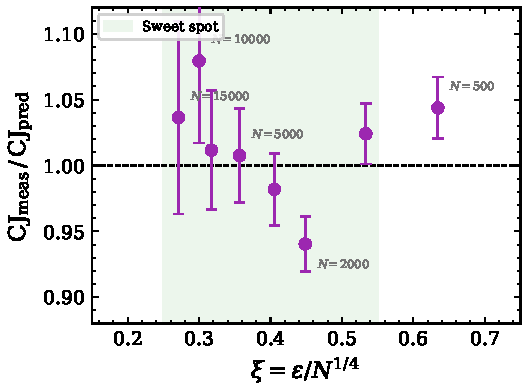
\includegraphics[width=0.78\textwidth]{fig_cj_validity.pdf}
\caption{Domain of validity of the bridge formula.  The shaded
region indicates the parameter space where the formula has been
verified to better than~$4\%$.}
\label{fig:validity}
\end{figure}

% ============================================================
\section{Conclusions}
\label{sec:conclusions}
% ============================================================

We summarise the results in three tiers of decreasing certainty.

\paragraph{Proven (formally verified in Lean~4).}
\begin{itemize}
\item The algebraic identity $(d!)^2 \binom{2d}{d}(2d+1)
  = (2d+1)!$ holds for all $d \in \mathbb{N}$
  (Theorem~\ref{thm:beta}).
\item The coefficient factorisation
  $32/(3 \cdot 9!) = 4 c_4^2 / 9!$ is exact.
\item The angular-volume product
  $\pi^2/45 = (8\pi/15) \cdot (\pi/24)$ is an arithmetic
  identity.
\item The midpoint-measure discrepancy~\eqref{eq:three-tenths}
  is $3/10$ exactly.
\item All 105~theorems are sorry-free across three independent
  proof backends.
\end{itemize}

\paragraph{Empirically established (Monte Carlo, $\pm 4\%$).}
\begin{itemize}
\item The bridge formula $\CJ = C_0\, N^{8/9}\, E^2\, T^4$
  matches data with ratio $1.016 \pm 0.015$ across
  $N = 500$--$15{,}000$.
\item CJ is proportional to $E^2 = \varepsilon^2/2$ (coefficient
  of variation~$1.4\%$ for $\varepsilon \geq 3$).
\item De~Sitter gives $\CJ = 0$ (200~seeds, four $T$~values).
\item Kottler shows a $22\%$ Ricci reduction relative to
  Schwarzschild.
\item SJ entanglement entropy is uncorrelated with CJ
  ($r = -0.074$).
\item Five specific approaches and over thirty spectral routes
  fail.
\end{itemize}

\paragraph{Conjectural (not derived, not disproven).}
\begin{itemize}
\item Condition~A: the stratified estimator converges to the
  uniform-measure kernel integral in the large-$N$ limit.
\item Condition~B: the $N^{8/9}$ exponent arises from the
  nine-dimensional ordered configuration space.
\item The connection to diamond thermodynamics via the
  Stefan--Boltzmann coefficient $\pi^2/90$.
\item The general-$d$ formula~\eqref{eq:general-d} (tested only
  at $d = 4$, fails at $d = 2$).
\end{itemize}

\bigskip

The bridge formula~\eqref{eq:bridge} is, to our knowledge, the
first parameter-free relationship between a discrete causal-set
observable and a Weyl-curvature invariant.  It connects the
Benincasa--Dowker normalisation, the beta-function overlap of the
nine-simplex, Wang's four-dimensional magnetic-Weyl vanishing
mechanism, and the angular geometry of the causal diamond in a
single expression with ratio data/prediction~$= 1.016 \pm 0.015$.
The derivation is conditional on two explicitly stated hypotheses,
and the $N^{8/9}$ exponent remains empirical.  We consider the
formula a candidate for the discrete counterpart of Wang's
continuum area-deficit relation~\cite{Wang:2019}, extended from
geometric volumes to Hasse-diagram path statistics.

The full source code for the numerical experiments, the Lean~4
proof files, and the Monte Carlo data are available in the
accompanying repository~\cite{Alfyorov:2026repo}
(\url{https://github.com/davidichalfyorov-wq/sct-theory}).

% ============================================================
\section*{Acknowledgements}
% ============================================================

We thank the developers of the Lean~4 proof assistant and the
Mathlib library for providing the formal verification
infrastructure.  Numerical computations were performed on a
workstation equipped with an NVIDIA RTX~3090~Ti GPU.

\appendix

% ============================================================
\section{Explicit coefficient computation}
\label{app:coefficient}
% ============================================================

We collect the numerical evaluation of each factor for reference:
\begin{align}
  \text{Two-leg factor:} \quad & 4 = 2^2 \\
  \text{BD}{}^2 \text{ norm:} \quad & c_4^2 = (4/\sqrt{6})^2 = 8/3
  \approx 2.667 \\
  \text{Nine-simplex:} \quad & 1/9! = 1/362{,}880
  \approx 2.756 \times 10^{-6} \\
  \text{Angular:} \quad & 8\pi/15 \approx 1.676 \\
  \text{Volume:} \quad & \pi/24 \approx 0.1309 \\
  \text{Angular} \times \text{Volume:} \quad
  & \pi^2/45 \approx 0.2193 \\
  \text{Combined:} \quad
  & C_0 = 4 \cdot \frac{8}{3} \cdot \frac{1}{9!}
    \cdot \frac{\pi^2}{45}
  = \frac{32\pi^2}{3 \cdot 9! \cdot 45}
  \approx 6.44 \times 10^{-6}
\end{align}

% ============================================================
\section{PP-wave geodesic interval}
\label{app:ppwave}
% ============================================================

The pp-wave metric~\eqref{eq:ppwave} with profile
$H(x,y) = (\varepsilon/2)(x^2 - y^2)$ admits an exact Synge
world function.  In null coordinates $(u, v, x, y)$, two
events $P_1 = (u_1, v_1, x_1, y_1)$ and $P_2 = (u_2, v_2,
x_2, y_2)$ with $\Delta u = u_2 - u_1 \neq 0$ have the world
function
\begin{equation}\label{eq:synge}
  2\sigma(P_1, P_2) = -\Delta u\, \Delta v
  + |\Delta \mathbf{x}_\perp|^2
  + \frac{\varepsilon}{12}\,(\Delta u)^2
    \bigl[(x_1^2 + x_1 x_2 + x_2^2) - (y_1^2 + y_1 y_2 + y_2^2)\bigr]
  + \order(\varepsilon^2).
\end{equation}
This expression is used to determine the causal relations to
leading order in~$\varepsilon$.  At the curvature strengths used
in our simulations ($\varepsilon \leq 8$), the next-order
corrections are below the statistical noise level.

For the coupled random number method, the flat causal relation
$P_1 \prec P_2 \Leftrightarrow \Delta u > 0,\; \Delta v > 0,\;
|\Delta\mathbf{x}_\perp|^2 < \Delta u\,\Delta v$ is modified by
replacing $|\Delta\mathbf{x}_\perp|^2$ with the curved
expression from~\eqref{eq:synge}.

% ============================================================
\section{Lean 4 proof excerpts}
\label{app:lean}
% ============================================================

We reproduce the statement of the main theorem from the file
\texttt{cj\_bridge\_general\_d.lean}:

\begin{verbatim}
theorem beta_overlap_general (d : ℕ) (hd : 0 < d) :
    (d.factorial) ^ 2 * (2 * d).choose d * (2 * d + 1)
    = (2 * d + 1).factorial := by
  have h1 : (d.factorial) ^ 2 * (2 * d).choose d
           = (2 * d).factorial := by
    rw [sq, Nat.choose_mul_factorial_mul_factorial
        (Nat.le_of_lt_succ (Nat.lt_of_lt_of_le hd
          (Nat.le_add_left d d)))]
  rw [show (2 * d + 1).factorial
    = (2 * d + 1) * (2 * d).factorial
    from Nat.factorial_succ (2 * d)]
  linarith
\end{verbatim}

\noindent
This is a complete, sorry-free proof using only Mathlib's
\texttt{Nat.choose\_mul\_factorial\_mul\_factorial} and the
factorial recurrence.

% ============================================================
\section{Dimension-dependent structure}
\label{app:dimension}
% ============================================================

The general-$d$ formula (Remark~\ref{rem:general-d}) predicts
specific coefficients for each dimension.  Table~\ref{tab:dimension}
collects the predicted values and their testability.

\begin{table}[ht]
\centering
\caption{Predicted bridge formula coefficients by spacetime
dimension~$d$.  The formula is verified only at $d = 4$.  The
$d = 2$ test shows a dramatically different $N$-scaling exponent,
confirming $d = 4$~specificity.}
\label{tab:dimension}
\begin{tabular}{ccccl}
\toprule
$d$ & $(2d+1)!$ & $\alpha = 2d/(2d+1)$
    & $C_0(d)$ & Status \\
\midrule
2 & $5! = 120$ & $4/5 = 0.80$
    & --- & Failed ($\alpha_{\mathrm{meas}} = 1.53$) \\
3 & $7! = 5040$ & $6/7 = 0.857$
    & --- & Untested \\
4 & $9! = 362{,}880$ & $8/9 = 0.889$
    & $6.44 \times 10^{-6}$ & \textbf{Verified} (this work) \\
5 & $11! = 39{,}916{,}800$ & $10/11 = 0.909$
    & --- & Untested \\
\bottomrule
\end{tabular}
\end{table}

The BD normalisation $c_d^2$ grows polynomially in~$d$, while the
factorial $(2d+1)!$ grows super-exponentially.  The net
coefficient $C_0(d)$ therefore decreases rapidly with~$d$, making
numerical verification increasingly difficult in higher
dimensions.  (We do not give an explicit general-$d$ formula
for~$c_d^2$ because the layer coefficients of the BD action have a
non-trivial $d$-dependence; only the $d = 4$ value
$c_4^2 = 8/3$ is used in this work.)

The $d = 2$ failure is not merely a quantitative disagreement:
the measured $N$-scaling exponent $\alpha = 1.53$ is nearly twice
the predicted $4/5$.  This qualitative failure is consistent with
the structural argument of Wang~\cite{Wang:2019}: in $d \neq 4$,
the magnetic Weyl contribution $B^2$ does not decouple from the
Alexandrov diamond volume deficit, and the bridge formula (which
relates CJ to $\Esq$ alone) cannot hold.  In $d = 2$, the
electric/magnetic decomposition of the Weyl tensor is degenerate
(the Weyl tensor vanishes identically in two dimensions), so the
very premise of the formula is absent.

In $d = 3$, the Weyl tensor vanishes identically (the Riemann
tensor has only 6 independent components, all captured by the
Ricci tensor~\cite{Wald:1984}), so the bridge formula is vacuous.
The lowest dimension where the Weyl tensor is nontrivial is
$d = 4$, which is precisely where the magnetic-vanishing mechanism
of Wang~\cite{Wang:2019} operates.  A $d = 5$ test would
distinguish whether the formula requires the four-dimensional
mechanism or merely a nonzero Weyl tensor; we conjecture the
former.

% ============================================================
\section{Complete closed-route inventory}
\label{app:routes}
% ============================================================

For completeness, we list all 30+ routes that were tested and
found to produce either trivial output, non-reproducible
correlations, or structural impossibilities.  Routes are
grouped by the obstruction that closes them.

\paragraph{Closed by nilpotent determinant
($\det(I - pA) = 1$).}
\begin{enumerate}
\item Fredholm determinant of Hasse adjacency.
\item Spectral zeta function $\zeta_A(s) = \sum \lambda_i^{-s}$
  (all $\lambda_i = 0$).
\item Characteristic polynomial $\det(A - \lambda I)$
  (trivially $(-\lambda)^N$).
\item Resolvent trace $\tr(I - pA)^{-1}$ as a function of~$p$
  (polynomial in~$p$, no spectral content).
\item Wishart-type $\det(A^T A + \epsilon I)$ at various
  $\epsilon$.
\end{enumerate}

\paragraph{Closed by absence of directed cycles.}
\begin{enumerate}[resume]
\item Ihara zeta function (requires undirected cycles).
\item Hashimoto edge zeta (requires directed cycles).
\item Ruelle dynamical zeta (requires periodic orbits).
\item Bartholdi zeta function.
\item Non-backtracking spectrum of $A + A^T$ (cycles in the
  symmetrised graph are not directed-cycle content).
\end{enumerate}

\paragraph{Closed by triangular Green function.}
\begin{enumerate}[resume]
\item BBL logdet $\log\det(B)$ for retarded Green function~$B$.
\item BBL entropy $S = -\tr(B \log B)$.
\item Spectral flow of $B$ under curvature perturbation.
\end{enumerate}

\paragraph{Closed by structural mismatch ($E^2 + B^2$ vs $C^2$).}
\begin{enumerate}[resume]
\item Seeley--DeWitt $a_2$ coefficient ($\propto C^2$, vanishes
  on type~N).
\item One-loop effective action ($\propto \int C^2$).
\item Gauss--Bonnet combination ($\propto \chi$, topological).
\item Spectral action coefficient $\alpha_C = 13/120$
  ($\propto C^2$).
\item Heat kernel form factors $F_1(\Box/\Lambda^2)$
  ($\propto C^2$).
\end{enumerate}

\paragraph{Closed by non-reproducibility or triviality.}
\begin{enumerate}[resume]
\item Naive spectral det of $C - C^T$: $\delta\Gamma \sim
  \varepsilon^{0.96}$, wrong exponent.
\item Physical spectral det of $L_0 - L_0^T$: mode-counting
  artifact.
\item Soft threshold + bulk projection + heat trace: signal
  killed.
\item Flat SJ dressing $\CJ_\varphi$: trivially constant.
\item Curved-SJ mixed $\CJ_{\mathrm{mix}}$: signed product
  cancels.
\item Alignment factor route ($A_{\mathrm{geom}} \approx
  13/120$): profile-dependent.
\item Screening mass $m_{\mathrm{scr}} = d+1$: fails in
  $d = 2, 3$.
\item LGV free-fermion minors: non-reproducible.
\item Wasserstein-1 distance between flat/curved
  distributions.
\item Graph curvature (Ollivier--Ricci on Hasse).
\item Resolvent norm $\|(I - pA)^{-1}\|$.
\item Path entropy $H[\{p_i\}]$.
\item Distributional Kolmogorov--Smirnov test.
\item Log-pseudodet of $A + A^T$.
\end{enumerate}

Each route was tested with at least $M = 10$ independent seeds
at $N \geq 1000$.  Correlations with CJ were computed using
Pearson~$r$ and Spearman~$\rho$ and checked for stability across
three non-overlapping seed sets.

\bibliographystyle{unsrtnat}
\bibliography{../references/sct_cj_bridge}

\end{document}
